\documentclass[a4paper,10pt]{article} 
\usepackage[a4paper,margin=1in]{geometry} 
\usepackage{adjustbox} 
\usepackage{algorithm}
\usepackage{algpseudocode}  
\usepackage{cite}
\usepackage{amsmath,amssymb,amsfonts}
\usepackage{graphicx}
\usepackage{textcomp}
\usepackage{subcaption}
\usepackage{xcolor}
\usepackage{xparse}       
\usepackage{url}
% \usepackage{algorithmic}
\usepackage{tikz}
\usepackage{booktabs}
\usepackage[normalem]{ulem}
\usepackage{float}

\newcommand\oak[1]{\textcolor{red}{OAK: #1}}
\newcommand{\new}[1]{\textcolor{blue}{#1}}

\title{Investigating the Coexistence of Security and Real-Time Availability in Resource-Constrained Devices}
\author{Amarin Laohajirapan}
\date{August 2025}

\begin{document}

\maketitle

\begin{abstract}
Internet-of-Things (IoT) and embedded devices are increasingly deployed
in mission-critical applications where both \emph{security} and
\emph{real-time availability} are essential. However, achieving these
two properties simultaneously on resource-constrained devices remains
challenging, as existing security mechanisms typically require
disabling system-wide interrupts to ensure atomicity, which can prevent
time-sensitive tasks from meeting their deadlines.

This thesis investigates the coexistence of security mechanisms and
real-time availability through four contributions. First, we propose a
taxonomy that classifies existing security mechanisms into dedicated
tasks and instrumentation-based integration, and analyze how each
degrades real-time availability. Second, as a case study, we present
the first port and systematic evaluation of SMARM (Shuffled Measurements
Against Roving Malware) on commodity RTOSes. Our design leverages ARM
TrustZone-M in place of the seL4 microkernel, retaining the same
security guarantees while enabling deployment on FreeRTOS and Zephyr.
We introduce the \emph{Frequency Accuracy Ratio} (FAR) metric to quantify
real-time impact, and show on the STM32L552ZE platform that SMARM
preserves FAR~$\approx 1.0$ only for block sizes $B \leq 1024$~bytes.

Third, we propose an \emph{atomic copy} enhancement that shifts the
non-interruptible window from hash computation to memory copy, improving
FAR from~$0.74$ to nearly~$1.0$ at $B = 1024$~bytes. However, this
reveals a new bottleneck: maintaining FAR~$\approx 1.0$ requires small
block sizes, which substantially increase secure-storage overhead.
Fourth, we propose \emph{SMARM+}, comprising SMARM+PRNG
that reduces storage from $O(n \log n)$ to $O(n)$ bits, and
SMARM+FPE that eliminates permutation storage entirely
via format-preserving encryption. At $B = 1024$~bytes,
SMARM+PRNG achieves a $9\times$ storage reduction with
7\% runtime overhead, while SMARM+FPE achieves a
$36\times$ reduction at 48\% additional runtime. Both variants preserve
SMARM's security guarantees and real-time behavior.

\noindent\textbf{Keywords:} Remote Attestation, Real-Time Systems,
TrustZone-M, RTOS, Shuffled Measurement, IoT Security
\end{abstract}


\section{Introduction}

\subsection{Background and Motivation}

Embedded devices, cyber-physical systems, and Internet-of-Things (IoT)
gadgets have become an integral part of modern society. They are widely
deployed in many real-life domains such as smart healthcare, industrial
automation, autonomous vehicles, and smart infrastructure. Recent
estimates indicate that the number of connected IoT devices worldwide
is approaching 20~billion as of 2025~\cite{statista2025iot}, reflecting
their pervasive role in daily life and critical services.

This rapid adoption, however, has also attracted malicious actors seeking
to compromise these systems, making their security a pressing global
concern in recent years~\cite{abera2016things}. Unlike conventional
computing platforms, IoT and embedded devices are typically
resource-constrained: they operate with limited processing power, memory,
and energy budgets, which precludes the deployment of sophisticated
security mechanisms such as commercial anti-virus software. As a result,
lightweight security primitives — including remote attestation,
control-flow integrity monitoring, and trusted execution environments —
have emerged as essential tools for defending these devices against
software compromise.


Beyond security, many of these devices also operate in real-time environments, such as braking systems in autonomous vehicles or medical devices monitoring patient health~\cite{abera2016things}. In such settings, meeting strict real-time deadlines is critical, as even minor delays can have serious safety consequences. For example, a small delay in a braking system could prevent an autonomous vehicle from stopping in time, leading to a crash; similarly, a delayed response in a medical device could put a patient's life at risk.

Despite the importance of both security and real-time operations, achieving them simultaneously on resource-constrained devices remains challenging. Existing security mechanisms commonly rely on disabling system-wide interrupts while performing security-critical operations. This ensures complete execution of such operations without interference from malware. However, this strategy conflicts with real-time requirements, as disabling interrupts prevents time-sensitive tasks from executing during that period, potentially causing the system to miss its deadlines.


\subsection{Problem Statement}

Although disabling interrupts is widely used to ensure atomicity in security mechanisms, the extent to which this practice affects real-time availability has not been systematically studied on commodity embedded platforms. Existing security mechanisms \cite{eldefrawy2012smart,nunes2019vrased,eldefrawy2017hydra,li2017epoxy,nunes2019aces,nunes2021pistis,wang2022mytee} have largely focused on security guarantees, often without measuring their impact on time-sensitive tasks running on the same device.
Recent work~\cite{joianeto2026iccad} has shown that this conflict has a cumulative dimension as well: atomic secure execution blocks periodic SysTick interrupts from reaching the RTOS, causing its internal clock to drift from real time over successive invocations. This means that the real-time impact is not limited to individual non-interruptible windows but can accumulate over long-running deployments.
Among existing approaches, SMARM~\cite{carpent2018smarm} attempts to reduce this conflict by shortening the non-interruptible period from the entire attestation duration to a single block measurement. However, SMARM has only been evaluated on the seL4 microkernel~\cite{klein2009sel4} — a platform with limited industrial deployment — leaving its practicality on widely-adopted RTOSes such as FreeRTOS~\cite{freertos2025} and Zephyr~\cite{zephyr2024} unverified. Furthermore, it is unclear whether SMARM can truly coexist with real-time workloads on commodity hardware, and whether its design imposes additional resource constraints (e.g., on secure storage) that limit its use on memory-constrained devices.
This thesis addresses the following research question: 
to what extent can existing security mechanisms — particularly 
remote attestation — coexist with strict real-time requirements 
on resource-constrained IoT devices, and how can such mechanisms 
be enhanced to better satisfy both properties simultaneously?

\subsection{Research Objectives}

To address the research question above, this thesis pursues the
following objectives:

\begin{enumerate}
    \item To systematically classify and analyze existing security
    mechanisms for resource-constrained devices with respect to their
    impact on real-time availability.
    
    \item To realize and evaluate SMARM on commodity RTOS-based platforms
    using ARM TrustZone-M as the trust anchor, and to quantify its
    real-time compatibility under realistic workloads.
    
    \item To propose enhancements to SMARM that further improve real-time
    availability and reduce secure-storage overhead, while preserving
    its original security guarantees.
    
    \item To provide deployment guidance for selecting among the proposed
    schemes based on real-time and secure-memory constraints of the
    target platform.
\end{enumerate}


\subsection{Scope and Limitations}

This thesis focuses on the following scope:


\begin{itemize}
    \item \textbf{Hardware platform.} All experiments are conducted on
    the STM32L552ZE Nucleo-144 development board~\cite{stm32l552},
    which features an ARM Cortex-M33 microcontroller with TrustZone-M
    security extensions. Although the design principles generalize to
    other Cortex-M33 platforms, generalization to other architectures
    (e.g., RISC-V, Cortex-A) is not investigated.
    
    \item \textbf{Operating systems.} We evaluate our work on two
    widely-adopted RTOSes: FreeRTOS and Zephyr. Other RTOSes (e.g.,
    NuttX, ThreadX) are not considered.
    
    \item \textbf{Security mechanism.} While our taxonomy covers
    multiple categories of security mechanisms, our enhancement work
    focuses on remote attestation, specifically the SMARM family of
    shuffled-measurement schemes.
    
    \item \textbf{Threat model.} We adopt the same threat model as
    SMARM~\cite{carpent2018smarm}: an adversary that fully controls
    the Non-Secure world software, including Knowledge of Future Volume
    (KFV) malware. Hardware/physical attacks, side-channel attacks,
    and Denial-of-Service (DoS) attacks are out of scope.
    
    \item \textbf{Real-time evaluation.} We focus on a single real-time
    task running alongside the attestation service. Multi-task
    schedulability analysis (e.g., deadline miss rate, worst-case
    execution time) is left as future work. We also do not analyze
    the cumulative RTOS time drift caused by atomic Secure-world
    execution, which is studied in detail in~\cite{joianeto2026iccad}.
\end{itemize}


\subsection{Contributions}

Motivated by the difficulty of fulfilling both security and real-time
requirements simultaneously, this thesis makes the following
contributions.

\begin{itemize}
    \item \textbf{Systematic Problem Investigation.} We propose a
    taxonomy that classifies existing security mechanisms for
    resource-constrained devices into two broad categories: dedicated
    security tasks and instrumentation-based integration. Based on
    this taxonomy, we analyze how interrupt-disabled operations in
    each category affect real-time task execution, identifying
    scenarios where real-time requirements are violated and
    highlighting the limitations of current security work.

    \item \textbf{Port and Evaluation of SMARM on RTOS.} As a case study,
    we present the first port of SMARM~\cite{carpent2018smarm} to
    commodity RTOS platforms. Our design leverages ARM
    TrustZone-M~\cite{trustzone2025} as the trust anchor in place of
    the seL4 microkernel~\cite{klein2009sel4}, retaining SMARM's
    original security guarantees while enabling deployment on
    widely-used RTOSes. To quantify the impact of SMARM on
    real-time task execution, we introduce the \emph{Frequency
    Accuracy Ratio (FAR)}, a metric that measures how closely a
    real-time task maintains its intended execution rate during
    attestation. We evaluate our port under FreeRTOS and Zephyr
    across multiple real-time workload classes, revealing that SMARM
    preserves FAR~$\approx 1.0$ only for block sizes
    $B \leq 1024$~bytes.

    \item \textbf{Atomic Copy Enhancement.} Through experiments on
    real hardware, we identify scenarios where SMARM still fails to
    meet real-time requirements. To address this, we propose an
    enhanced version of SMARM that reduces the non-interruptibility
    period by shifting the atomic operation from hash computation to
    memory copy. We empirically demonstrate that our enhancement
    achieves FAR~$\approx 1.0$ at block sizes where the original
    SMARM yields only FAR~$\approx 0.74$. This enhancement, however,
    reveals a new practical bottleneck: achieving FAR~$\approx 1.0$
    requires small block sizes, which substantially increase the
    secure-storage overhead for the shuffled permutation, limiting
    deployment on memory-constrained TrustZone-M devices.

    \item \textbf{SMARM+: Storage-Efficient Shuffled Attestation.}
    To address the secure-storage bottleneck identified above, we
    propose \emph{SMARM+}, a family of enhanced SMARM variants.
    SMARM+PRNG replaces the explicit permutation 
    array with a compact bitmap and a pseudorandom number generator 
    (PRNG), reducing, reducing secure-storage requirements
    from $O(n \log n)$ to $O(n)$ bits. SMARM+FPE
    eliminates permutation storage entirely by deriving the
    measurement order at runtime using format-preserving
    encryption~\cite{bellare2009fpe,dworkin2016sp800}, requiring only
    $O(1)$ secure memory. Both variants preserve SMARM's security
    guarantees and real-time behavior while substantially reducing
    secure-storage overhead, enabling practical deployment on
    platforms with highly constrained Secure RAM.
\end{itemize}


\subsection{Thesis Organization}

The remainder of this thesis is organized as follows.
Chapter~\ref{ch:literature} reviews existing security mechanisms for
resource-constrained devices, examines SMARM and its follow-on studies
in detail, and identifies the research gaps that motivate this work.
Chapter~\ref{ch:methodology} describes the experimental platform,
system architecture, and methodology used throughout this thesis,
including our port of SMARM to FreeRTOS and TrustZone-M, the design
of the atomic copy enhancement, and the SMARM+ variants.
Chapter~\ref{ch:eval-smarm} presents the experimental evaluation of
the security taxonomy and our SMARM realization on commodity RTOS
platforms, identifying the storage--real-time tension that motivates
subsequent contributions. Chapter~\ref{ch:atomic-copy} evaluates the
atomic copy enhancement and demonstrates its improvement in real-time
availability, while also identifying the secure-storage bottleneck.
Chapter~\ref{ch:smarmplus} presents the experimental evaluation of
SMARM+, including secure-storage reduction, runtime overhead, and
deployment guidance across different Secure-RAM scenarios. Finally,
Chapter~\ref{ch:conclusion} summarizes the contributions of this
thesis, discusses its limitations, and outlines directions for
future research.




\section{Literature Review}
\label{ch:literature}
This chapter reviews existing work related to the core challenges addressed 
in this thesis. We begin by surveying security mechanisms for resource-constrained 
devices and examining how their atomicity requirements conflict with real-time 
availability (Section~2.1). We then provide background on the foundations of 
remote attestation and control-flow attestation (Section~2.2), followed by a 
review of recent work that aims to reconcile attestation with real-time 
constraints, including interruptible attestation designs and studies of
cumulative RTOS time drift during atomic secure execution (Section~2.3).
Next, we focus on SMARM~\cite{carpent2018smarm}, 
the primary mechanism studied in this work, along with its follow-on studies 
(Section~2.4). Finally, we identify the research gaps that motivate the 
contributions of this thesis.

\subsection{Security Mechanisms in Constrained Devices}

We classify existing security mechanisms for resource-constrained devices into two categories: (1) those that require having a dedicated task to handle security operations and (2) those that embed security operations within existing tasks via software instrumentation.

\subsubsection{Security Mechanisms with Dedicated Tasks}
This category encompasses mechanisms that operate as dedicated tasks scheduled alongside application tasks. 
For example, SMART~\cite{eldefrawy2012smart}, VRASED~\cite{nunes2019vrased} and HYDRA~\cite{eldefrawy2017hydra} propose remote attestation architectures that convince a remote verifier that a prover (i.e., an embedded device) is installed with correct software; their techniques rely on using a dedicated attestation task that securely computes a software measurement and an attestation report.

APEX~\cite{apex} and SLAPP~\cite{slapp} enable the verifier to assess that a specific function has executed correctly on the prover, with the execution as well as a proof of this execution performed/computed in a standalone task. 
DIALED~\cite{dialed} extends APEX by additionally incorporating data-flow information into this dedicated execution.

We observe that many of these mechanisms adopt a common approach: to achieve their respective security goals, this dedicated task must be executed atomically, without interruption; otherwise, malware may interfere with this task, leading to a compromise of the security guarantees.
For example, in SMART, if interrupts are not disabled, malware may preempt the attestation task and relocate itself during the measurement to evade detection from the verifier.
Similarly, in APEX, malware can interrupt the execution of a verifier-requested function and prevent it from successful completion, either by resuming execution at a different location or by modifying intermediate data values, while still being able to produce a valid proof of execution.

Due to this reason, these mechanisms enforce the atomicity requirement by disabling system-wide interrupts during execution of their dedicated security-critical task. 
The duration of interrupt disablement depends on the execution time of the security task, which can be significant in practice (e.g., 0.45 seconds for VRASED~\cite{nunes2019vrased}). 
Thus, time-sensitive tasks are prevented from running for a noticeable amount of time, making these mechanisms unsuited in real-time settings.




\subsubsection{Security Mechanisms Integrated into Existing Tasks via Instrumentation}
This category embeds security operations directly into application task execution through compiler or source-level instrumentation, rather than having them as separate tasks~\cite{li2017epoxy,nunes2019aces,nunes2021pistis,wang2022mytee}. 

Examples of this category include EPOXY~\cite{li2017epoxy}, ACES~\cite{nunes2019aces}, PISTIS~\cite{nunes2021pistis}, and MyTEE~\cite{wang2022mytee}. 

EPOXY~\cite{li2017epoxy} proposes a technique to provide an isolated execution environment for privileged code in embedded systems.
It leverages LLVM to instrument programs with secure privilege elevation, enabling restricted operations (e.g., I/O access) to be executed in a sandbox environment.
We observe that, to be secure, this instrumented code must execute atomically; otherwise, an adversary could interrupt execution after the privilege is elevated and inject malicious code~\cite{li2017epoxy}.
Therefore, EPOXY requires interrupts to be disabled during the execution of its instrumented code~\cite{li2017epoxy}.

Similarly, MyTEE~\cite{wang2022mytee} proposes to instrument programs to perform privilege elevation to build a trusted execution environment (TEE). It therefore inherits the same requirement: its instrumented code must execute with interrupts disabled~\cite{wang2022mytee}.

ACES~\cite{nunes2019aces} introduces a compartmentalization technique for embedded systems.
It enforces isolation between compartments by instrumenting the program binary to configure the memory protection unit (MPU) at compartment boundaries~\cite{nunes2019aces}.
However, we note that the security of ACES relies on the instrumented code correctly setting up the MPU. 
If an interrupt occurs during this configuration, the MPU may not be properly enforced, breaking the security guarantee~\cite{nunes2019aces}. 
Therefore, it is implicit from its design that interrupt disablement must happen during execution of ACES instrumented code~\cite{nunes2019aces}.

PISTIS~\cite{nunes2021pistis} instruments virtualized instructions into existing code to implement root-of-trust functionalities in embedded systems, such as remote attestation, memory isolation, and secure software updates~\cite{nunes2021pistis}.
Similar to ACES and EPOXY, its instrumented code performs security operation at runtime (e.g., validating a memory write) and must therefore execute uninterrupted~\cite{nunes2021pistis}.
As a result, PISTIS also requires interrupts to be disabled during the execution of its instrumented code~\cite{nunes2021pistis}.

Overall, instrumentation-based approaches still require interrupts to be disabled during the execution of instrumented code~\cite{li2017epoxy,nunes2019aces,nunes2021pistis,wang2022mytee}.
This can degrade the system's real-time availability, a phenomenon that will be further explored in this thesis~\cite{li2017epoxy,nunes2019aces,nunes2021pistis,wang2022mytee}.



\subsection{Foundations of Remote Attestation}

This section provides background on remote attestation (RA) and
related security mechanisms for resource-constrained devices. We
first survey the evolution of RA schemes from software-based to
hardware-assisted approaches, then discuss control-flow
attestation techniques that build upon RA principles.

\subsubsection{Remote Attestation: Background and Evolution}

Remote attestation is a security technique that allows a trusted
verifier to detect malware on a remote device (called the prover)
by verifying the integrity of its software state. In a typical RA
protocol, the verifier sends a challenge to the prover, which then
computes a measurement---usually a cryptographic hash of its
memory---and returns it as evidence. The verifier compares this
evidence against a known-good reference to determine whether the
prover is compromised~\cite{kuang2022survey}.

Early RA schemes were purely software-based. Pioneer~\cite{seshadri2005pioneer}
proposed one of the first software-based attestation techniques,
using precise timing constraints to detect malware on legacy
systems. However, software-only approaches require tight timing
bounds and are vulnerable to various attacks in
Survey of remote attestation in IoT generally covers the
evolution from software-based to hybrid schemes, including
the limitations of purely software-based approaches in
resource-constrained settings~\cite{ankergard2021software,kuang2022survey}. To address these limitations,
subsequent work explored hybrid and hardware-assisted designs.

Francillon et al.~\cite{francillon2014minimalist} proposed a
minimalist approach to remote attestation that reduces the
hardware requirements for the prover, making RA more practical for
low-end devices. Brasser et al.~\cite{brasser2016remote} examined
RA from the prover's perspective, analyzing the assumptions and
limitations that affect the feasibility of RA on constrained
platforms.

Hardware-assisted RA schemes provide stronger security guarantees
by relying on a trusted execution environment (TEE) or a minimal
root of trust. TrustLite~\cite{koeberl2014trustlite} introduced a
security architecture for tiny embedded devices that supports
memory isolation without requiring a full memory management unit.
TyTAN~\cite{brasser2015tytan} extended this idea by providing a
tiny trust anchor specifically designed for resource-constrained
IoT devices. Among modern hardware platforms, ARM
TrustZone-M~\cite{trustzone2025} provides a lightweight TEE for
microcontroller-class devices by partitioning hardware resources
into Secure and Non-Secure worlds, enabling security-critical
operations to execute in isolation from potentially compromised
application software. Luo et al.~\cite{luo2022trustzone} presented a
comprehensive security analysis of TrustZone-M-based IoT systems,
identifying runtime software vulnerabilities---including buffer
overflows, format string attacks, and return-oriented
programming---and demonstrating that despite the hardware-level
isolation, the security of the overall system still depends on
careful implementation of the Secure World software.

\subsubsection{Control-Flow Attestation}

Beyond basic memory integrity verification, control-flow
attestation (CFA) extends RA to verify not only what code is
present on the device, but also the execution path taken by a
program. C-FLAT~\cite{abera2016cflat} proposed the first CFA scheme
for embedded systems, recording a trace of control-flow transfers
during program execution and attesting this trace to a verifier.
This enables detection of control-flow hijacking attacks that may
not modify the code itself but alter its execution order.

Subsequent work improved CFA efficiency through hardware support.
LO-FAT~\cite{lo-fat} reduced CFA overhead by using hardware
performance counters to record control-flow events at low cost.
LiteHAX~\cite{litehax} proposed a lightweight hardware-assisted
attestation mechanism that minimizes the trusted computing base
while maintaining detection coverage. ATRIUM~\cite{atrium}
introduced runtime attestation resilient against memory attacks,
operating continuously rather than on-demand to detect transient
malware.

Despite their effectiveness, these CFA schemes share a common
limitation with the RA mechanisms discussed earlier: they require
interrupts to be disabled during the measurement process to ensure
the integrity of the control-flow trace. This creates the same
tension with real-time availability that motivates this thesis.


\subsection{Toward Interruptible and Real-Time Attestation}

The previous sections established that virtually all existing RA and CFA mechanisms require interrupts to be disabled during security-critical operations, creating a fundamental conflict with real-time availability. This section reviews recent work that specifically attempts to reconcile security with real-time requirements. We discuss approaches that aim to make attestation interruptible, followed by broader frameworks for co-designing security and real-time systems.

\subsubsection{Reconciling RA with Safety-Critical Operation}

The tension between remote attestation and safety-critical operation was first explicitly identified in a DAC invited paper by Carpent et al.~\cite{reconciling-ra}, which discussed the challenges of ensuring both secure attestation and continuous availability on simple IoT devices. The authors observed that existing RA techniques either require on-demand and atomic operation, which can harm safety-critical functions, or risk failing to detect transient and self-relocating malware when those requirements are relaxed. They proposed mitigation strategies including periodic self-measurements, interruptible attestation through shuffled memory traversals, and memory locking mechanisms~\cite{reconciling-ra}. This work laid the conceptual foundation for subsequent interruptible attestation schemes.

Building on this idea, ERASMUS~\cite{erasmus} introduced a self-measurement approach where the prover periodically measures its own memory without requiring an explicit challenge from the verifier. By performing self-measurement, ERASMUS reduces the need for on-demand attestation sessions that must execute atomically. However, it still relies on a trusted execution environment and does not fully eliminate the atomicity requirement during the measurement itself~\cite{erasmus}.

\subsubsection{Interruptible Attestation Designs}

More recent works have proposed concrete RA designs that support interrupts during attestation. IDA~\cite{ida2024} introduced a hybrid attestation method that removes the requirement for disabling interrupts by using a trusted hardware monitoring module to verify the attestation process. Instead of relying on a secret key to compute the attestation response, IDA certifies the attestation's authenticity based on whether the process was followed correctly. An extension, IDA+, further tracks program memory changes between attestation requests or during interrupts, enabling detection of TOCTOU (time-of-check-time-of-use) attacks~\cite{ida2024}. We note that while IDA successfully eliminates the need for interrupt disablement, it requires additional hardware monitoring logic, which may not be available on all commodity platforms. We
note that TOCTOU attacks are a well-known challenge in
remote attestation, as analyzed by Nunes et al.~\cite{nunes2021toctou},
and IDA+ is among the first hybrid schemes to explicitly
address this attack vector.

ISC-FLAT~\cite{isc-flat} addresses the conflict between control-flow attestation and real-time operations by leveraging ARM TrustZone-M as the trust anchor. To the best of our knowledge, it is the first TEE-based CFA approach that can securely support interrupts while maintaining CFA integrity. ISC-FLAT achieves this by isolating the effects of external interrupts from the execution being attested within the Secure World. However, it is designed specifically for CFA rather than memory integrity attestation, and thus addresses a different but related problem~\cite{isc-flat}.

ASAP~\cite{asap} proposes a different strategy: it supports asynchronous real-time operations during proofs of execution by allowing the prover to suspend an ongoing proof, service an interrupt, and resume the proof afterward. This is designed for scenarios where real-time tasks must execute even while the system is in the middle of producing an attestation report. We observe that ASAP focuses on proofs of execution rather than memory integrity attestation, and its applicability to SMARM-style shuffled measurement remains an open question~\cite{asap}.

CHARM~\cite{perfcounter-ra} uses hardware performance counters on the prover side and machine learning on the verifier side to make interruptible RA feasible for constrained microcontrollers. Rather than requiring atomic execution, CHARM allows interrupts to occur during the measurement and relies on the verifier to distinguish benign interrupt activity from malware behavior based on the performance counter traces. This approach introduces a new trade-off: it requires the verifier to maintain an ML model for each prover and is sensitive to changes in the interrupt profile caused by legitimate system updates~\cite{perfcounter-ra}.

\subsubsection{Security and Real-Time Co-Design Frameworks}

A complementary line of work proposes scheduling-level approaches to co-design security and real-time constraints, rather than focusing on individual attestation mechanisms. Mishra et al.~\cite{mishra2022survey} conducted a survey of control-flow integrity techniques specifically for real-time embedded systems and found that very few CFI mechanisms are designed with real-time constraints in mind. The authors identified this gap and called for future research that leverages real-time execution characteristics---such as predictable task release patterns---to inform CFI design~\cite{mishra2022survey}.

Extending this direction, RECFISH~\cite{mishra2023procrastinating} proposed a CFI framework that exploits the predictable release pattern of periodic real-time systems to perform CFI checks as security tasks that can be scheduled alongside application tasks. This framework allows CFI verification to be deferred to safe points without affecting real-time deadlines, effectively decoupling the timing of security checks from application execution. We note that while RECFISH addresses the schedulability aspect of security, it is designed for CFI rather than remote attestation, and it requires a trusted scheduler to coordinate the security tasks~\cite{mishra2023procrastinating}.

At a higher level, Kansal et al.~\cite{kansal2023integrated} proposed an integrated real-time and security scheduling framework for cyber-physical systems. Their approach uses an n-dimensional security matrix to model the available defense mechanisms and transforms the problem of maximizing security subject to schedulability into a variant of the knapsack problem. This enables system designers to select the best combination of security mechanisms while ensuring that real-time deadlines are still met~\cite{kansal2023integrated}.


\subsubsection{RTOS Time Drift During Atomic Secure Execution}

A complementary dimension of the conflict between atomic
secure services and real-time availability was recently
characterized by Joia Neto et al.~\cite{joianeto2026iccad}.
This work identifies that when the Secure World executes a
trusted computing service atomically on TrustZone-M (i.e.,
with Non-Secure interrupts disabled), it blocks the periodic
SysTick interrupt from reaching the Non-Secure RTOS.
Because the Nested Vectored Interrupt Controller~(NVIC) can
buffer only one pending SysTick expiration, multiple
consecutive expirations are silently discarded while the
Secure service is running. As a result, the RTOS undercounts
the number of ticks that have elapsed, causing its internal
clock to drift from real time.

The authors formalize this phenomenon through a tick-loss
model. For a SysTick period $T_{\mathrm{tick}}$ and an atomic
section of duration $A_i$, the number of lost ticks per
invocation is:
\begin{equation}
    \Delta_i(\phi_i) = \max\left(0,\;
    \left\lceil\frac{\phi_i + A_i}{T_{\mathrm{tick}}}\right\rceil
    - 1\right),
\end{equation}
where $\phi_i$ is the offset from the last delivered tick.
Over multiple invocations, the cumulative drift grows
linearly with both the frequency of atomic operations and
the number of tick periods they span~\cite{joianeto2026iccad}.

The work evaluates four trusted computing services ---
control-flow integrity (CFI), software-fault isolation (SFI),
remote attestation, and authenticated hot-patching --- on both
FreeRTOS and Zephyr running on a Cortex-M33 platform
(Figure~\ref{fig:rtos-systick-loss}).  The results show that
each remote attestation invocation introduces up to 238~ms of
drift on FreeRTOS and 202~ms on Zephyr, while the larger
atomic window of hot-patching produces nearly 2.9~seconds of
drift per invocation~\cite{joianeto2026iccad}.

\begin{figure}[H]
    \centering
    \includegraphics[width=0.85\linewidth]{tick_miss.png}
    \caption{SysTick loss during atomic Secure-world execution.}
    When the Secure service runs with interrupts disabled,
    multiple SysTick expirations are lost because the NVIC can
    buffer only one pending event. Figure adapted
    from~\cite{joianeto2026iccad}.
    \label{fig:rtos-systick-loss}
\end{figure}

To address this problem, Joia Neto et al.~\cite{joianeto2026iccad}
propose a Secure-driven time synchronization mechanism that
redirects SysTick handling to the Secure World during atomic
execution. The Secure World maintains a trusted monotonic
time reference, captures each SysTick expiration, and updates
the Non-Secure tick data structures on behalf of the RTOS.
When the atomic service completes, the RTOS resumes with a
tick counter that already accounts for all ticks that occurred
while its own handler was precluded from running. This
approach restores correct timekeeping without requiring any
modifications to the RTOS or application code and is
orthogonal to the block-level interrupt period studied in the
context of SMARM~\cite{joianeto2026iccad}.

Although this work addresses a different facet of the
conflict --- cumulative time drift rather than per-block
non-interruptibility --- it highlights that the consequences
of atomic secure execution extend beyond the immediate
blocking of application tasks. In long-running deployments,
even brief atomic operations that occur frequently can
produce schedulable drift that degrades real-time performance
over time. This observation reinforces the practical severity
of the problem that this thesis addresses and motivates the
need for attestation mechanisms that minimize both per-event
interference and long-term side effects on RTOS timekeeping.

Despite these advances, none of the works discussed in this section addresses all of the dimensions that we target in this thesis: supporting shuffled-measurement attestation on commodity RTOS platforms, evaluating real-time compatibility under realistic workloads, and reducing secure-storage overhead. The interrupted attestation approaches (IDA, ISC-FLAT, ASAP, CHARM) all introduce additional hardware requirements or are designed for different forms of attestation. The scheduling frameworks (RECFISH, Kansal et al.) operate at the system level and do not address the unique challenges of shuffled-measurement attestation. This motivates our focus on SMARM and its storage-efficient enhancements in the following sections.


\subsection{SMARM and Its Follow-on Studies}
As discussed in Section 2.1, existing remote attestation frameworks require interrupts to be disabled while the prover computes a measurement~\cite{eldefrawy2012smart,nunes2019vrased,eldefrawy2017hydra}. 
This can prevent time-sensitive tasks from executing, making those tasks unavailable for non-negligible amounts of time, e.g., up to 0.45 seconds in VRASED~\cite{nunes2019vrased}.
SMARM~\cite{carpent2018smarm} addresses this issue by proposing to compute the measurement in a \textbf{randomized} order, determined by a one-time secret permutation derived from the verifier's challenge and a pre-shared secret key. 
To protect the permutation from tampering by untrusted software, it must be securely stored on the prover device or protected through cryptographic means, such as authenticated encryption~\cite{carpent2018smarm}. 
This randomized approach reduces the likelihood that roving malware can reliably relocate itself to evade detection during attestation~\cite{carpent2018smarm}.
In terms of real-time availability, SMARM reduces the non-interruptible period from the entire attestation measurement to a single block measurement, allowing interrupts after each block is measured~\cite{carpent2018smarm}. 
This introduces a trade-off in choosing the block size in SMARM: smaller blocks shorten the non-interruptible period, improving application task availability.
However, this also increases the number of blocks to measure, resulting in a larger (secure) storage for the permutation data. 
Conversely, larger blocks reduce storage overhead but increase the non-interruptible period, potentially impacting real-time task execution~\cite{carpent2018smarm}.


\paragraph{SMARM Workflow.}
Figure~\ref{fig:smarm_workflow_4phases} illustrates the end-to-end 
operation of SMARM. Upon receiving a fresh challenge $\mathit{chal}$ 
from the verifier, the prover's secure execution environment performs 
the attestation through four sequential phases.


\begin{figure}[H]
    \centering
    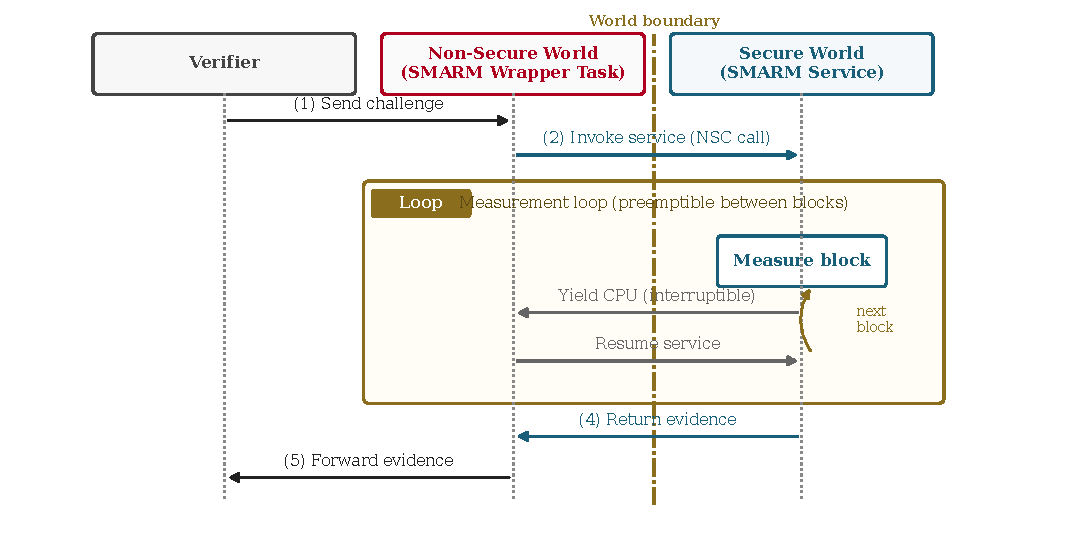
\includegraphics[width=0.7\linewidth]{smarm_workflow.pdf}
    \caption{Operational workflow of SMARM, consisting of four phases:
    Permutation Generation, Atomic Block Measurement, Loop Check, and 
    Finalization. Figure adapted from~\cite{carpent2018smarm}.}
    \label{fig:smarm_workflow_4phases}
\end{figure}


\textbf{Phase 1: Permutation Generation.}
The prover generates a one-time permutation $\sigma$ over the block 
indices $\{0, 1, \ldots, n-1\}$, where $\sigma(i)$ specifies which 
memory block is measured at iteration~$i$. To ensure that $\sigma$ is 
both fresh and private for each attestation instance, SMARM derives 
the PRNG seed from a secure hash of the verifier's challenge 
$\mathit{chal}$ and a pre-shared secret key~$k$:
\begin{equation}
\sigma = \text{FisherYates}(\text{Hash}(\mathit{chal}, k), 
[0, \ldots, n-1])
\end{equation}
The Fisher--Yates shuffle algorithm~\cite{fisher1938statistical} 
produces a uniformly random permutation in $O(n)$ time, making it 
well-suited for resource-constrained devices. Once generated, 
$\sigma$ is stored in secure storage that is inaccessible to 
untrusted software.

\textbf{Phase 2: Atomic Block Measurement.}
At each iteration~$i$, the prover retrieves the next block index 
$\sigma(i)$ from secure storage, disables system-wide interrupts, 
and incrementally updates an HMAC computation with the contents of 
block $M_{\sigma(i)}$. After the block measurement completes, 
interrupts are re-enabled. The atomic window is therefore limited 
to a single block measurement rather than the entire memory region.

\textbf{Phase 3: Loop Check.}
The prover checks whether all $n$ blocks have been measured. If 
not, control returns to Phase~2 to measure the next block in the 
shuffled order; otherwise, execution proceeds to Phase~4.

\textbf{Phase 4: Finalization.}
After all blocks have been measured, the prover finalizes the HMAC 
computation using the secret key~$k$, producing the attestation 
evidence. This evidence is transmitted to the verifier, which can 
independently reconstruct $\sigma$ using its copy of $k$ and 
$\mathit{chal}$, recompute the expected measurement, and validate 
the received evidence.

\paragraph{Security Requirements.}
To achieve its security goals, SMARM relies on a secure execution 
environment that satisfies three architectural requirements. We 
adopt these requirements throughout this thesis as the baseline 
security guarantees that any SMARM realization must preserve:

\begin{itemize}
    \item \textbf{(S1) Controlled execution.} The attestation code 
    can be invoked and exited only through well-defined entry and 
    exit points, preventing partial execution or mid-code entry by 
    malicious code. Within the attestation code, interrupts may be 
    re-enabled only between consecutive block measurements, never 
    during a single measurement.

    \item \textbf{(S2) Key secrecy.} The attestation key~$k$ is 
    accessible exclusively to the attestation code and must remain 
    inaccessible to all other software components on the prover.

    \item \textbf{(S3) Private measurement order.} The permutation 
    $\sigma$ that determines the measurement order must be stored in 
    memory inaccessible to untrusted software, ensuring that KFV 
    malware cannot predict which block will be measured next.
\end{itemize}

In its original prototype, SMARM realizes this secure execution 
environment using the HYDRA architecture~\cite{eldefrawy2017hydra}, 
which leverages the formally verified seL4 
microkernel~\cite{klein2009sel4} as its trust anchor. The attestation 
logic is implemented as an isolated user-space task whose memory 
(including~$k$ and~$\sigma$) is inaccessible to other tasks, 
satisfying~(S2) and~(S3). Entry to this task is restricted to a 
single dedicated IPC endpoint, and the task is initially scheduled 
at the highest priority to prevent preemption during a block 
measurement, satisfying~(S1).



\begin{figure}[H]
    \centering
    \includegraphics[width=0.85\linewidth]{smarm_hydra.pdf}
    \caption{The original SMARM prototype atop the HYDRA architecture.
    The measurement task executes in seL4's user space and is isolated 
    from other tasks through capability-based access control. The 
    attestation key~$k$ and permutation~$\sigma$ reside exclusively 
    within the measurement task's memory. Figure adapted 
    from~\cite{carpent2018smarm}.}
    \label{fig:smarm_hydra_prototype}
\end{figure}


SMARM considers adversaries with three different levels of knowledge, as summarized in Table~\ref{tab:smarm-adversary}.

\begin{table}[h]
    \centering
    \resizebox{\textwidth}{!}{%
        \begin{tabular}{|l|p{10cm}|}
        \hline
        \textbf{Adversary Knowledge} & \textbf{Description} \\ \hline
        Knowledge of Future Volume (KFV) & Malware only knows how many blocks remain to be measured (e.g., through timing information). \\ \hline
        Knowledge of Future Coverage (KFC) & Malware knows which blocks have already been measured, possibly through side-channel observations. \\ \hline
        Knowledge of Future Order (KFO) & Malware knows the exact future measurement order, for example due to permutation leakage. \\ \hline
        \end{tabular}
    }
    \caption{Adversary knowledge considered in SMARM's security analysis~\cite{carpent2018smarm}.}
    \label{tab:smarm-adversary}
\end{table}

It was concluded that the KFV adversary is the most realistic, while KFC and KFO require knowledge of the permutation order and thus are more far-fetched since its confidentiality is protected by the secure storage or the authenticated encryption~\cite{carpent2018smarm}. 
In this thesis, we adopt the same assumption and consider only the KFV adversary.

Nonetheless, a KFV adversary may attempt to evade SMARM by relocating itself after each block measurement. The authors of~\cite{carpent2018smarm} analyze this scenario and show that the success probability of such an evasion strategy is limited to $(1-1/n)^n$ for $n$ memory blocks.
For large $n$, this approaches $e^{-1}\approx 37\%$~\cite{carpent2018smarm}.
To achieve more reliable detection, SMARM recommends performing multiple rounds of independent measurements. 
For example, after 7 rounds the evasion probability becomes less than $10^{-3}$, and after 13 rounds, less than $10^{-6}$~\cite{carpent2018smarm}.
We note that all existing experimental results for SMARM have been obtained solely on the seL4 microkernel~\cite{klein2009sel4}, and its real-time performance and effectiveness on widely used platforms such as FreeRTOS -- especially in the context of embedded and TrustZone-M-based devices as considered in this thesis -- remain an open research question. 
This motivates our porting and evaluation work, which aims to clarify SMARM's practical viability in real-time embedded settings.




\subsubsection{Follow-on Studies and Extensions}
Several follow-on studies have extended the idea introduced by SMARM, each addressing specific challenges in remote attestation for embedded and IoT devices while retaining some of SMARM's core limitations and trade-offs~\cite{aman2021prom,aman2018hatt}.



Passive Remote Attestation (PRoM)~\cite{aman2021prom} applies the concept of shuffled measurement to multi-core IoT devices, designed to counter roving malware in environments with parallel execution, which are considerably more complex than single-core architectures~\cite{aman2021prom}. This approach divides the device memory into multiple blocks and distributes the attestation of these blocks across different cores for parallel processing~\cite{aman2021prom}. As a result, PRoM significantly reduces attestation time and improves system availability compared to techniques such as SMARM, which require hashing every block of memory sequentially~\cite{aman2021prom}.

However, PRoM still faces important limitations regarding interrupt handling~\cite{aman2021prom}. While it does not require interrupts to be disabled throughout the entire attestation period in a fully atomic manner, as in SMART or traditional hybrid RA, PRoM must still disable interrupts during the measurement of each batch of blocks (i.e., memory is divided into blocks, and interrupts are disabled only while a batch is being measured)~\cite{aman2021prom}. Therefore, compared to other techniques, PRoM greatly reduces the negative impact on system availability, but it still cannot fully support unrestricted interrupt handling during the entire attestation process.

HAtt~\cite{aman2018hatt} aims to increase the availability in IoT devices by using physical unclonable functions (PUFs) to secure secrets and adopting the randomized measurement approach~\cite{aman2018hatt}. Similar to SMARM, HAtt mandates that the attestation code for measuring any single block execute without interruption -- even though the broader protocol is more availability-friendly than classical schemes~\cite{aman2018hatt}. This requirement for block-level atomicity means that HAtt cannot provide full interruptibility throughout the attestation process~\cite{aman2018hatt}.


{ITERATOR~\cite{sponziello2025iterator} adopts a different strategy to reduce 
secure storage overhead. In an offline phase, it constructs a Cuckoo filter over all 
memory blocks to represent the valid software state. During runtime, ITERATOR 
incrementally verifies memory through two interleaved operations: \textsc{Attest}, 
which validates a newly selected block against the filter, and \textsc{Check}, which 
re-validates a set of previously measured blocks to defend against relocation malware. 
Although ITERATOR reduces permutation storage complexity to $O(n)$ through 
Cuckoo filters, it still requires interrupts to remain disabled during each consecutive 
\textsc{Attest}--\textsc{Check} sequence, meaning non-interruptible execution is not 
eliminated. Furthermore, its actual storage overhead depends on implementation 
parameters such as the target false-positive rate and load factor, resulting in a larger 
constant cost in practice compared to storing $n$ bits exactly as in our proposed 
approach.

Despite the advancement made by these follow-on studies, none have fully resolved 
the fundamental trade-off between atomic (i.e., uninterruptible) attestation and 
real-time device availability~\cite{aman2021prom,aman2018hatt}. In practice, all 
require either uninterruptible phases or additional hardware to mitigate attack risk 
during attestation, illustrating the persistent challenges in achieving both robust 
security and uninterrupted service in constrained IoT 
environments~\cite{carpent2018smarm,aman2021prom,aman2018hatt}. 
{Moreover, none of these works have been implemented on RTOS platforms 
or evaluated under real-time workloads, and all inherit SMARM's secure-storage 
limitation, which can become prohibitive on memory-constrained devices.


Table~\ref{tab:related-work-comparison} summarizes the key differences 
between our work and prior shuffled-measurement remote attestation schemes 
across four dimensions: RTOS support, real-time evaluation, hardware independence, 
and secure storage complexity.

\begin{table}[h]
\centering
\caption{Comparison of shuffled-measurement remote attestation schemes.
$\checkmark$ = satisfied, $\times$ = not satisfied.}
\label{tab:related-work-comparison}
\resizebox{\textwidth}{!}{%
\begin{tabular}{lcccc}
\hline
\textbf{Work} & \textbf{RTOS Support} & \textbf{RT Evaluation} 
& \textbf{No Extra HW} & \textbf{Secure Storage} \\
\hline
SMARM~\cite{carpent2018smarm}       & $\times$ & $\times$ & $\checkmark$ & $O(n \log n)$ \\
PRoM~\cite{aman2021prom}            & $\times$ & $\times$ & $\checkmark$ & $O(n \log n)$ \\
HAtt~\cite{aman2018hatt}            & $\times$ & $\times$ & $\times$     & $O(n \log n)$ \\
ITERATOR~\cite{sponziello2025iterator} & $\times$ & $\times$ & $\checkmark$ & $O(n)$    \\
\hline
SMARM+PRNG (ours)   & $\checkmark$ & $\checkmark$ & $\checkmark$ & $O(n)$ \\
SMARM+FPE (ours)    & $\checkmark$ & $\checkmark$ & $\checkmark$ & $O(1)$ \\
\hline
\end{tabular}
}
\end{table}

As shown in Table~\ref{tab:related-work-comparison}, our work is the first 
to simultaneously address all four dimensions: deploying shuffled attestation on 
commodity RTOS platforms, evaluating real-time compatibility under realistic 
workloads, avoiding additional hardware dependencies, and substantially reducing 
secure-storage requirements. Prior works satisfy at most two of these four criteria.


\subsubsection{Research Gaps and Motivation}
Despite significant advances in remote attestation for embedded systems, particularly through SMARM and subsequent extensions, four critical gaps persist that limit the practical deployment of secure attestation in real-time embedded environments.  


The first gap lies in the \textbf{incomplete resolution of the fundamental trade-off} between security and availability. Although SMARM improves upon fully atomic approaches such as SMART and VRASED by allowing interrupts between memory blocks, it still requires disabling interrupts during the measurement of each block. This creates non-interruptible execution windows that risk violating real-time deadlines. Subsequent approaches share this limitation: PRoM relies on atomic batch processing across multiple cores, HAtt enforces block-level atomicity despite using PUFs, and IDA~\cite{ida2024}, while supporting interrupt handling during attestation, introduces additional hardware complexity that reduces its feasibility for many embedded deployments. This pattern across generations of research shows that 
achieving both strong security guarantees and continuous 
real-time availability remains an open problem.


The second gap concerns the \textbf{limited platform validation and deployment scope}. SMARM has been evaluated exclusively on the seL4 microkernel, leaving its practical effectiveness on more widely adopted platforms such as FreeRTOS entirely unverified. This gap is significant because seL4 and FreeRTOS differ substantially in scheduling policies, interrupt handling mechanisms, memory management, and deployment patterns. Whereas seL4 relies on capability-based scheduling and benefits from formal verification, FreeRTOS is built on priority-based preemptive scheduling with simpler memory management and dominates industrial embedded applications. Without systematic evaluation on FreeRTOS, SMARM's improvements in real-time availability have not been 
verified for the majority of real-world embedded systems.

The third gap arises from insufficient analysis under realistic real-time workloads. Existing evaluations of SMARM and related approaches have not thoroughly investigated their impact on high-frequency tasks that require the overall system to be highly available. 
Moreover, the influence of attestation-induced delays on task synchronization, resource contention, and schedulability remains poorly understood. These omissions are critical because even brief delays in real-time systems can lead to deadline violations and, in the worst cases, 
system-level failures.

The fourth gap concerns the \textbf{unaddressed secure-storage overhead} 
inherent in shuffled-measurement schemes. SMARM and all of its follow-on studies 
require storing a full permutation $\sigma$ of size $n \cdot \lceil \log_2 n \rceil$ bits 
in secure memory, where $n$ is the number of memory blocks. Achieving real-time 
compatibility (FAR~$\approx 1.0$) requires small block sizes, which increase $n$ and 
thus the storage demand substantially — ranging from 576 bytes at $B = 1024$ bytes 
to approximately 13~KB at $B = 64$ bytes on our target platform. On TrustZone-M 
devices, Secure RAM is strictly limited and must often be shared with other 
security-critical services such as confidential inference~\cite{islam2023confidential}, 
control-flow integrity monitoring~\cite{kawada2021tzmcfi}, and secure key 
storage~\cite{silabs2020an1271}. Dedicating a significant fraction of Secure RAM 
solely to the permutation array can therefore render SMARM impractical in 
multi-service deployments, even when real-time requirements are otherwise satisfied. 
This gap motivates the design of storage-efficient alternatives that preserve 
SMARM's security and real-time guarantees.}

\section{Research Methodology}
\label{ch:methodology}
This chapter describes the experimental methodology used throughout this 
thesis. We begin by presenting the hardware platform and software simulation 
approach used in all experiments. We then describe the system architecture and 
the two categories of security mechanisms evaluated. Next, we detail our port of 
SMARM to FreeRTOS and TrustZone-M, including the block size tradeoff analysis 
that motivates subsequent contributions. Finally, we present the design of the 
atomic copy enhancement and the SMARM+ variants; their experimental 
evaluation is presented in Chapters~\ref{ch:atomic-copy} and~\ref{ch:smarmplus}, respectively.

\subsection{Experimental Platform and Setup}

\subsubsection{Hardware Configuration}

We selected the STM32L552ZE development board~\cite{stm32l552}, featuring a 110 MHz ARM Cortex-M33 MCU, 512 KB Flash, and 256 KB SRAM, as our experimental platform. This device represents a widely deployed class of resource-constrained IoT controllers that must support both real-time responsiveness and security-sensitive operations~\cite{abera2016things}. Despite advanced security features such as Arm TrustZone hardware isolation~\cite{trustzone2025} and ultra-low-power operation, it still shares common limitations with simpler embedded systems, 
including limited memory bandwidth, interrupt latency, 
and resource contention between security operations and application tasks~\cite{koeberl2014trustlite}.

Figure~\ref{fig:hardware_setup} shows our experimental setup consisting of the STM32L552ZE development board connected to a laptop via UART for data collection. The UART connection operates at 115200 baud rate and serves as the communication channel for logging execution timing data and system events. Python scripts running on the laptop collect the data streams for analysis.

\begin{figure}[H]
\centering
\includegraphics[width=0.8\linewidth]{hardware_setup.jpg}
\caption{STM32L552ZE development board connected to laptop via UART for data collection}
\label{fig:hardware_setup}
\end{figure}

\subsubsection{Application Task Simulation}


In our experiments, we simulate application task workloads using a cycle-based busy-wait loop written in inline assembly~\cite{francillon2014minimalist}.
This approach creates controlled computational loads that consume CPU time for precise durations, enabling the study of how interrupt-disabled security operations affect various simulated real-time tasks~\cite{brasser2016remote}.


\begin{algorithm}
\caption{\_busy\_cycles delay loop (used when interrupts are disabled)}
\begin{algorithmic}[1]
\Require cycles: Number of clock cycles to delay
\State \texttt{iterations} $\gets$ (cycles + 2) / 3
\State Inline assembly block begins:
\State \quad Align loop to 4-byte boundary
\State \quad Label: \texttt{1:}
\State \quad Subtract 1 from \texttt{iterations}
\State \quad If result is not zero, branch to label \texttt{1}
\State \quad Inline assembly block ends
\Ensure Precise delay loop even when interrupts are disabled
\end{algorithmic}
\end{algorithm}


The simulated application tasks execute this loop at regular intervals to emulate periodic real-time computations~\cite{freertos2025}. 
Execution timing data is continuously logged through UART timestamps, with external Python scripts collecting data to measure task frequencies and quantify security operation impact on application timing.


Having established the hardware foundation, we now examine the software architecture that coordinates security and application tasks on this platform.


\subsection{System Architecture}

As shown in Figure~\ref{fig:systemmodel}, our experimental system consists of three layers: hardware, kernel, and userland. We use FreeRTOS~\cite{freertos2025} as the kernel due to its widespread adoption in both academia and industry.
While formally verified kernels such as seL4~\cite{klein2009sel4} offer stronger theoretical guarantees, their deployment remains limited. 
In contrast, FreeRTOS reflects the dominant RTOS environment for commercial IoT and embedded devices, making it a relevant platform for evaluating practical feasibility. FreeRTOS handles scheduling of application tasks in the userland, and we provide a custom busy-wait loop as a kernel API to simulate timing-precise task execution.

In addition to FreeRTOS, we also evaluate our implementation under 
Zephyr~\cite{zephyr2024}, a modern open-source RTOS supported by the Linux 
Foundation. Zephyr differs from FreeRTOS in several respects relevant to our 
evaluation: it provides a more structured device driver model, supports Trusted 
Firmware-M (TF-M)~\cite{tfm2024} as its Secure-world runtime, and uses a 
different interrupt handling architecture. Including Zephyr allows us to assess whether 
our findings generalize across RTOS platforms, or whether they are specific to 
FreeRTOS scheduling behavior.

\begin{figure}[H]
\centering
\includegraphics[width=0.95\linewidth]{systemmodel.png}
\caption{Overall system model used in the experimental setup}
\label{fig:systemmodel}
\end{figure}


With the three-layer system model in place, we proceed to evaluate how different security integration approaches perform within this model.


\subsubsection{Evaluation of Security Categories}
We investigate existing security mechanisms by evaluating the two dominant categories identified in our literature review: (1) dedicated security tasks and (2) instrumentation-based integration. 
These categories represent a vast majority of approaches for implementing security operations in resource-constrained environments. 


To evaluate the impact of real-time availability in a given security mechanism, we propose a performance metric, called the \textit{Frequency Accuracy Ratio (FAR)} as follows:

\begin{equation}
    FAR = \frac{f_{\text{observed}}}{f_{\text{baseline}}}
    \label{eq:far}
\end{equation}

where $f_{\text{observed}}$ denotes the observed execution frequency 
of the real-time task $T_{RT}$, and $f_{\text{baseline}}$ denotes its 
frequency in the absence of interrupt-disabled security operations.

FAR represents the ratio between the observed task frequency in our experiments and the expected (theoretical) frequency.
A FAR value close to 1 indicates that the application task operates nearly at the expected frequency, reflecting high availability. 
Conversely, a low FAR value shows that the task runs less frequently than expected, indicating reduced real-time availability of the system.


Our experiments focus on non-preemptive scheduling, meaning tasks run to completion without interruption from other tasks. 
This ensures deterministic timing behavior and allows us to isolate the specific impact of interrupt-disabled periods during security operations on application task timing. This task division supports both dedicated security task approaches (where security operations run as separate tasks) and instrumentation-based integration (where security operations are embedded within application tasks).


We begin our security evaluation with the dedicated task approach, where security operations run as independent tasks separate from application tasks.

\subsubsection{Setup: Dedicated Security Tasks}
\label{sec:dedicated-setup}

\begin{figure}[H]
\centering
\includegraphics[width=0.9\columnwidth]{Dedicatedtask.png}
\caption{Dedicated security task experimental model showing temporal separation between security tasks (red) and application tasks (gray), with interrupt masking during security operations}
\label{fig:dedicatedtask}
\end{figure}

In the dedicated security task methodology, security operations are implemented as independent tasks, separated from normal application tasks~\cite{brasser2015tytan}. We deploy one security task and one application task, both running as a Normal World task scheduled using FreeRTOS. 
To emulate security-sensitive routines, the security task disables interrupts and executes the busy-wait loop described earlier, representing time-consuming atomic operations.

We carefully schedule the execution of secure and application tasks to prevent overlap, using a round-robin scheduling strategy in FreeRTOS.
Theoretically, this scheduling policy ensures that once a task (secure or application) begins execution, it runs to completion without being pre-empted by the other task, as illustrated in Figure~\ref{fig:dedicatedtask}.


\subsubsection{Instrumentation-Based Security Integration}
\label{sec:instrumentation-setup}

\begin{figure}[H]
\centering
\includegraphics[width=0.9\columnwidth]{SFITask.png}
\caption{Instrumentation-based integration model. Security operations (red) are embedded within the application task (gray) and are executed periodically during the task execution}
\label{fig:sfi_task}
\end{figure}

For the instrumentation-based methodology, each application-related task is instrumented to include a security operation before its main functional execution begins~\cite{li2017epoxy}. In this design, every time an instrumented code runs, it first executes a sequence that disables interrupts and performs the simulation loop to emulate security operation, such as verifying memory permissions or enforcing runtime policies, before returning to the application logic.



In this experiment, we schedule two application tasks running in the Normal World and schedule them in such a way that their execution will not pre-empt each other, as shown in Figure~\ref{fig:sfi_task}.
Each application task has security operations embedded directly within its code body, which are triggered periodically during its execution.
We use the simulation loop to emulate this (embedded) security operation as well as the normal application simulation.



\subsection{Case Study: SMARM}
After examining the problem of real-time availability in existing 
security mechanisms for embedded systems, we turn our attention to 
enhancing one such mechanism. In this thesis, we focus on 
SMARM~\cite{carpent2018smarm}, which addresses a key limitation in 
traditional remote attestation~\cite{eldefrawy2012smart}: the need 
for long non-interruptible periods that harm real-time availability. 
Traditional attestation computes a cryptographic measurement 
(e.g., HMAC) over the entire memory region atomically, disabling 
interrupts for the entire duration. SMARM instead divides memory 
into blocks and processes them in a randomized 
order~\cite{carpent2018smarm}, as shown in 
Algorithm~\ref{alg:smarm_baseline}.

\begin{algorithm}
\caption{ShuffledHMAC (baseline; no memcpy, disable around each hash update)}
\label{alg:smarm_baseline}
\begin{algorithmic}[1]
\Require $BLOCKS$, $BLOCK\_SIZE$, $shuffled\_indices[0..BLOCKS-1]$, $real\_memory$
\State \Call{HMAC\_Init}{hmac, key}
\For{$i \gets 0$ to $BLOCKS-1$}
  \State $blk \gets$ address of block at $shuffled\_indices[i]\cdot BLOCK\_SIZE$ in $real\_memory$
  \State \Call{DisableInterrupts}{}
  \State \Call{HMAC\_Update}{hmac, $blk$, $BLOCK\_SIZE$}
  \State \Call{EnableInterrupts}{}
\EndFor
\State \Call{HMAC\_Finalize}{hmac}
\Ensure digest is available in \textit{hmac.digest}
\end{algorithmic}
\end{algorithm}

The key innovation is that interrupts now can be disabled only during the hashing of each individual block, not the entire memory region. 
The randomized order (generated using a secure shuffle seeded with a verifier's challenge) prevents roving malware from predicting which memory blocks will be measured next, making evasion difficult.


\subsection{Challenges of Adapting SMARM to RTOS}
\label{sec:smarm-challenges}

This subsection discusses why a naive replacement of seL4 
with a commodity RTOS is insufficient to preserve SMARM's 
security guarantees, motivating our TrustZone-M-based design.

A straightforward approach would be to retain the HYDRA-based 
SMARM prototype and simply replace the seL4 microkernel with 
an RTOS kernel. However, this approach introduces critical 
security gaps. The original design relies on seL4's formally 
verified isolation to protect the measurement task and prevent 
untrusted tasks from accessing the attestation key $k$ and 
permutation $\sigma$~\cite{eldefrawy2017hydra}. Such guarantees are 
absent in commonly deployed RTOSes.

In vanilla FreeRTOS, all tasks execute at the same privilege 
level under bare-metal settings~\cite{freertos2025}, allowing 
any compromised task to freely read or modify $k$ and 
$\sigma$, breaking (S2) and (S3). Even RTOSes that offer 
optional memory isolation — such as FreeRTOS-MPU or Zephyr — 
do not provide formally verified isolation. In practice, these 
kernels have been shown to contain exploitable vulnerabilities; 
for example, CVE-2018-16525 enables remote code execution in 
FreeRTOS~\cite{freertos_cve}, and CVE-2024-6137 permits 
malicious writes to Zephyr's kernel memory~\cite{zephyr_cve}. 
An adversary exploiting such vulnerabilities can break 
isolation and compromise the measurement task entirely.

Therefore, simply replacing seL4 with an RTOS is insufficient 
to make SMARM secure. Our design instead leverages ARM 
TrustZone-M to provide hardware-enforced isolation on 
off-the-shelf embedded platforms, as described in the 
following subsection.

\subsubsection{Porting SMARM to FreeRTOS + TrustZone-M}
\label{sec:porting}

The original SMARM proposal was not evaluated under an RTOS, leaving its suitability for strict real-time requirements unclear. 
To assess SMARM under real-time systems, our first step is to port it to a popular RTOS—FreeRTOS. 
For security, we require the device to have TrustZone-M security extensions and implement the SMARM logic  inside the Secure World~\cite{trustzone2025}. 
The secure code constructs a SHA256 HMAC over shuffled memory blocks, with permutations seeded using cryptographically-derived values.
Communication between Secure and Normal worlds uses non-secure callable APIs. 

Unlike the original seL4 implementation~\cite{eldefrawy2017hydra} that relied on microkernel guarantees~\cite{klein2009sel4}, our FreeRTOS port uses TrustZone hardware isolation to maintain the same security properties. 
The shuffled permutation ($shuffle\_indices$) is stored in Secure World's memory, accessible only to the SMARM code, ensuring malware cannot predict the measurement order~\cite{carpent2018smarm}.


Therefore, our design decomposes SMARM into two components, as illustrated in Figure~\ref{fig:smarm_trustzone}:

\begin{itemize}
    \item \textbf{Wrapper Task.} A regular RTOS task executing in the Non-Secure 
    world. It serves as the interface between the verifier and the Secure-world SMARM 
    logic. Upon receiving an attestation request, it invokes the Secure Service and 
    forwards the returned evidence to the verifier. It runs at the lowest RTOS priority 
    to allow preemption by real-time tasks between block measurements.

    \item \textbf{Secure Service.} Resides entirely in the Secure world and is exposed 
    via a Non-Secure Callable~(NSC) entry point. It executes the SMARM logic 
    (Algorithm~\ref{alg:smarm_baseline}), disabling interrupts via the \texttt{CPSID} 
    instruction during each block measurement to enforce atomic execution. The 
    attestation key $k$ and permutation $\sigma$ are stored exclusively in Secure RAM, 
    satisfying~(S2) and~(S3).
\end{itemize}

Since the Secure Service satisfies all three security requirements~(S1)--(S3), our 
TrustZone-M-based realization retains the same security guarantees as the original 
SMARM design~\cite{carpent2018smarm}.

\begin{figure}[H]
\centering
\includegraphics[width=0.85\linewidth]{system-threat-model.pdf}
\caption{SMARM on RTOS using TrustZone-M: the Wrapper Task runs in the 
Non-Secure world while the Secure Service executes SMARM logic inside the 
Secure world, with hardware-enforced isolation provided by TrustZone-M.}
\label{fig:smarm_trustzone}
\end{figure}



The end-to-end interaction between the verifier and the SMARM 
components is illustrated in Figure~\ref{fig:smarm_workflow_tz}. 
Upon receiving a challenge, the Wrapper Task invokes the Secure 
Service via an NSC call. The Secure Service executes the SMARM 
logic: after each block measurement completes, execution returns 
to the Non-Secure world where the RTOS can preempt the Wrapper 
Task to schedule real-time tasks. After all blocks are measured, 
the Secure Service returns the attestation evidence to the Wrapper 
Task, which forwards it to the verifier.

\begin{figure}[H]
    \centering
    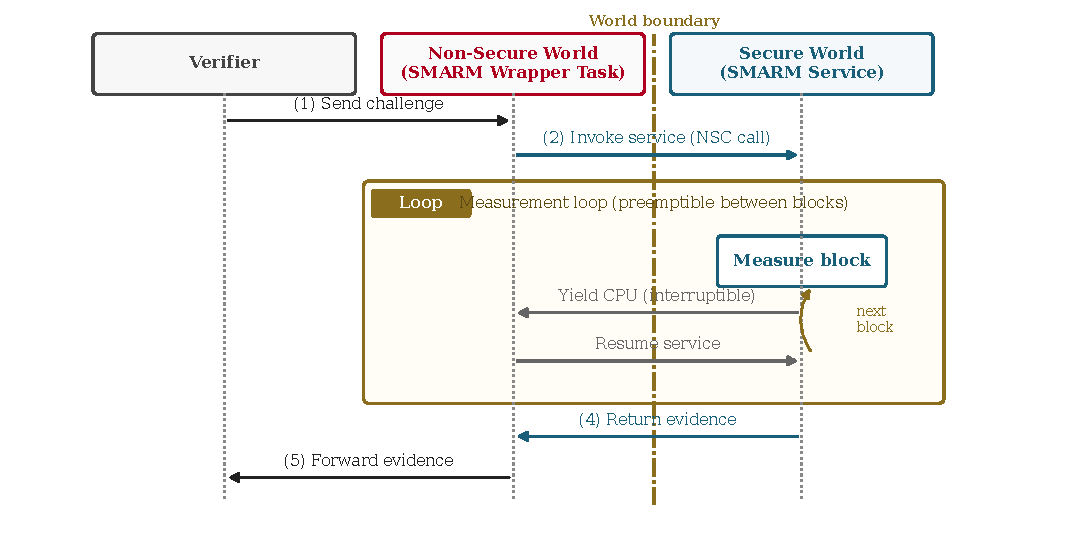
\includegraphics[width=0.85\linewidth]{smarm_workflow}
    \caption{End-to-end workflow of our TrustZone-M-based SMARM 
    realization. The Wrapper Task in the Non-Secure world interfaces 
    with the verifier, while the Secure Service executes SMARM logic 
    inside the Secure world. Real-time tasks may preempt the Wrapper 
    Task between consecutive block measurements.}
    \label{fig:smarm_workflow_tz}
\end{figure}



\subsubsection{Experimental Parameters}
After porting SMARM to RTOS, we evaluate its real-time availability using the FAR metric by considering different block sizes: 64, 128, 256, 512, 1024, 2048, and 4096 bytes, with total attested memory size set to 512 KB. The frequency of the application task is varied across multiple
real-time workload classes; the specific values are presented in
Chapter~\ref{ch:eval-smarm}. The application task uses
\texttt{osPriorityHigh}. The security task (SMARM) is always set to \texttt{osPriorityNormal}. Application tasks always have higher priority and will preempt the security task except when the SMARM protocol disables interrupts. The frequency of the security task is not fixed; it depends on how long each attestation takes and the chosen test parameters. All timing and frequency measurements are collected using cycle-accurate logging.


As described in Section~\ref{sec:porting}, SMARM exhibits a fundamental trade-off as block size varies: the non-interruptibility period
$t_{\text{disabled}}$ scales with block size, while the secure-storage
requirement $|\sigma| = n \cdot \lceil \log_2 n \rceil$ bits scales
inversely. Section~\ref{ch:eval-smarm} quantifies this trade-off
empirically and identifies its implications. This trade-off suggests two
complementary directions for improving SMARM on RTOS-based platforms.


\subsection{Design of Proposed Enhancements}
\label{sec:proposed-enhancements}

The block size trade-off identified in Chapter~\ref{ch:eval-smarm}
suggests two complementary directions for improving SMARM on RTOS-based
platforms. First, the non-interruptibility period $t_{\text{disabled}}$
grows linearly with block size, motivating a redesign that decouples the
atomic operation from cryptographic hashing. Second, the secure-storage
requirement $|\sigma| = n \cdot \lceil \log_2 n \rceil$ bits scales
unfavorably as block size decreases, motivating storage-efficient
alternatives to the explicit permutation array.

We address these two dimensions through two orthogonal contributions:

\begin{itemize}
    \item \textbf{Atomic copy enhancement} (Chapter~\ref{ch:atomic-copy})
    reduces $t_{\text{disabled}}$ by shifting the interrupt-disabled
    operation from hashing to memory copy, while preserving SMARM's
    security guarantees~(S1)--(S3).

    \item \textbf{SMARM+ family} (Chapter~\ref{ch:smarmplus}) reduces
    secure-storage overhead by eliminating the explicit permutation
    array. SMARM+PRNG reduces storage to $O(n)$ bits via
    a bitmap representation, while SMARM+FPE eliminates
    permutation storage entirely via format-preserving encryption,
    requiring only $O(1)$ secure memory.
\end{itemize}

Both contributions inherit the system model and TrustZone-M-based
realization described in Section~\ref{sec:porting}. The full design,
security analysis, and experimental evaluation of each contribution are
presented in their respective chapters.



\section{Evaluation of Security Mechanisms and SMARM}
\label{ch:eval-smarm}

This chapter presents the first systematic evaluation of SMARM on 
commodity RTOS-based platforms using ARM TrustZone-M as the trust 
anchor in place of the seL4 microkernel used in the original 
HYDRA-based prototype~\cite{eldefrawy2017hydra,carpent2018smarm}. 
Although our taxonomy in Chapter~\ref{ch:methodology} classifies 
existing security mechanisms into dedicated security tasks and 
instrumentation-based integration, our experimental evaluation 
focuses on SMARM as a representative case study, since it directly 
addresses the real-time availability problem through shuffled 
measurements and serves as the primary target of our subsequent 
enhancements (Chapters~\ref{ch:atomic-copy} and~\ref{ch:smarmplus}).

We begin by describing our SMARM implementation on the STM32 Nucleo-144 
development board, including the TrustZone-M-based design that 
preserves SMARM's original security guarantees. We then characterize 
the non-interruptibility period $t_{\mathrm{disabled}}$ across block 
sizes and RTOS choices, followed by an evaluation of real-time 
availability using the FAR metric under high, medium, and low real-time 
workloads. Finally, we identify a fundamental tension between 
secure-storage requirements and real-time availability, motivating 
the enhancements in subsequent chapters.

\subsection{SMARM on RTOS: Implementation}
\label{sec:smarm-impl}

We present the first port of SMARM to commodity RTOS-based platforms. 
Unlike the original HYDRA-based prototype that relied on the formally 
verified seL4 microkernel~\cite{klein2009sel4} for measurement-task 
isolation, our realization leverages ARM TrustZone-M as the trust 
anchor, enabling deployment on widely-adopted RTOSes such as FreeRTOS 
and Zephyr. The detailed design of this port — including the 
decomposition into a Non-Secure Wrapper Task and a Secure Service 
satisfying SMARM's original security requirements (S1)--(S3) — is 
described in Chapter~\ref{sec:porting}.

We implement our TrustZone-M-based SMARM realization on an STM32 
Nucleo-144 development board~\cite{stm32nucleo144}, equipped with an ARM 
Cortex-M33 MCU running at 110~MHz, 512~KB of flash storage, and 256~KB of 
SRAM with TrustZone-M support. In our configuration, 256~KB of flash and 
128~KB of SRAM are allocated to the Secure world, with the remaining memory 
assigned to the Non-Secure world.

On the software side, the Non-Secure world runs an unmodified RTOS compiled 
with size optimizations (\texttt{-Os}); our prototype supports both FreeRTOS 
and Zephyr. The SMARM Wrapper Task is implemented as a regular RTOS task 
in the Non-Secure world, consisting of \textit{115 lines} of C code. The 
Secure-world SMARM Service implements Algorithm~\ref{alg:smarm_baseline} 
using SHA-256 as the hash function for memory block measurement and 
HMAC-SHA256 to compute the attestation evidence. The Secure-world 
implementation consists of \textit{153 lines} of C code and contributes 
\textit{33,968 bytes} to the trusted computing base~(TCB).

The end-to-end interaction between the verifier and the SMARM 
components follows the workflow described in 
Chapter~\ref{sec:porting} (see Figure~\ref{fig:smarm_workflow_tz}).


\subsection{SMARM on RTOS: Non-Interruptibility Period}
\label{sec:smarm-noninterrupt}

We evaluate $t_{\text{disabled}}$ across block sizes
$B \in \{64, 128, 256, 512, 1024, 2048, 4096\}$ bytes, running SMARM
under both FreeRTOS and Zephyr. For each attestation block, interrupts
are disabled only for the duration of the SHA-256 hash computation over
that block:
\begin{equation}
    t_{\text{disabled}}(B) = \frac{B}{\text{Hash Throughput}}.
    \label{eq:tdisabled}
\end{equation}
The hash throughput depends on the hardware and the cryptographic
implementation; we measure it empirically on our target platform.
Each $t_{\text{disabled}}$ measurement below is averaged over five runs;
standard deviations are below 1\% in all cases.

Figure~\ref{fig:tdisabled} reports the results. As expected from
Equation~\ref{eq:tdisabled}, $t_{\text{disabled}}$ grows approximately
linearly with $B$, confirming that larger blocks lead to longer
non-interruptibility periods on our target device.
At $B = 64$ bytes, $t_{\text{disabled}}$ remains below 0.1\,ms across
both RTOSes. At $B = 4096$ bytes, it reaches approximately 3.8\,ms — a
period long enough to reduce FAR below 1.0 in high-frequency real-time
tasks.

FreeRTOS and Zephyr yield nearly identical $t_{\text{disabled}}$ values
across all block sizes. This indicates that the non-interruptibility
period is determined primarily by the SHA-256 hash computation cost over
each memory block, rather than RTOS-specific scheduling or context-switch
overhead. This finding is consistent with the fact that interrupts are
disabled during the hash computation, preventing any RTOS scheduler
activity during this window.

The results in this section characterize one side of the SMARM trade-off:
larger blocks increase $t_{\text{disabled}}$. Whether this translates
into actual real-time availability degradation depends on the workload
characteristics, which we examine in the next section. We
return to the full storage-vs-real-time trade-off in
Chapter~\ref{sec:storage-tension}.

\begin{figure}[H]
\centering
\includegraphics[width=0.85\linewidth]{tdisabledplot.pdf}
\caption{Non-interruptibility period $t_{\mathrm{disabled}}$ of our SMARM 
realization on the STM32 Nucleo-144 platform across block sizes $B$, for 
both FreeRTOS and Zephyr. Each point is averaged over five runs; standard 
deviations are below 1\%. $t_{\mathrm{disabled}}$ grows linearly with $B$, 
consistent with Equation~\ref{eq:tdisabled}.}
\label{fig:tdisabled}
\end{figure}


\subsection{SMARM on RTOS: Real-Time Availability}

\subsubsection{Experimental Setup}

To evaluate the impact of SMARM on real-time availability, we consider a 
simplified yet representative scenario in which SMARM runs alongside a 
single real-time task $T_{RT}$. Although our setup includes only one 
real-time task, it is intentionally conservative: our purpose is to identify 
the conditions under which SMARM and real-time execution fail to coexist. 
If coexistence does not hold in this simplified setting, it is unlikely to 
hold in more complex deployments with multiple real-time tasks.

We model three classes of practical real-time workloads by varying the 
frequency of $T_{RT}$:

\begin{itemize}
    \item \textbf{High real-time workload:} $T_{RT}$ runs at 1000~Hz, 
    representing control loops in robotic or automotive systems.
    \item \textbf{Medium real-time workload:} $T_{RT}$ runs at 100~Hz, 
    representing sensor sampling or network polling tasks.
    \item \textbf{Low real-time workload:} $T_{RT}$ runs at 10~Hz, 
    representing background monitoring or logging tasks.
\end{itemize}

We measure $f_{\mathrm{observed}}$ using the on-chip hardware cycle counter 
and convert cycles to time using the 110~MHz CPU clock. FAR is computed following Equation~\ref{eq:far} defined in
Chapter~\ref{ch:methodology}, where $f_{\mathrm{observed}}$ denotes 
the execution frequency of $T_{RT}$ when SMARM is active, and 
$f_{\mathrm{baseline}}$ denotes the frequency of $T_{RT}$ in the absence 
of SMARM-induced interrupt disablement. FAR = 1.0 indicates no 
interference from atomic block measurements; values below 1.0 indicate 
degraded real-time availability.


\subsubsection{Results}

Figure~\ref{fig:setup_and_baseline_far} reports FAR across different block 
sizes, real-time workloads, and RTOS choices. Across all configurations, we 
observe a consistent trend: \textbf{FAR remains close to 1.0 for 
$B \leq 1024$~bytes, but degrades noticeably as the block size increases 
beyond this threshold.}

At $B = 2048$~bytes, FAR decreases to approximately 0.55 on FreeRTOS and 
0.65 on Zephyr under medium and high real-time workloads, while remaining 
around 0.75 under low workloads. At $B = 4096$~bytes, FAR drops further 
to 0.27 on FreeRTOS and 0.32 on Zephyr across all workload settings, 
meaning that $T_{RT}$ executes at less than one-third of its intended 
frequency during attestation. These results confirm that SMARM cannot 
reliably preserve real-time availability at larger block sizes.

Both RTOSes show nearly identical FAR trends across all 
evaluated configurations, as visible across all three subfigures. This 
result suggests that the main source of real-time interference is 
SMARM's atomic block measurement — characterized by $t_{\mathrm{disabled}}$ 
— rather than RTOS-specific scheduling behavior such as context-switch 
latency or task prioritization policy. In particular, the block size $B$, 
which directly determines $t_{\mathrm{disabled}}$ as shown in 
Equation~\ref{eq:tdisabled}, is the main factor governing 
real-time availability in our evaluation.

We also note that FAR values are consistent across all three workload 
classes at a given block size, particularly for $B \geq 2048$~bytes. 
Comparing Figures~\ref{fig:baseline_results_1000hz}, 
\ref{fig:baseline_results_100hz}, and~\ref{fig:baseline_results_10hz}, 
the FAR curves overlap closely regardless of whether $T_{RT}$ runs at 
10~Hz, 100~Hz, or 1000~Hz. This suggests that once $t_{\mathrm{disabled}}$ 
is large enough to reduce FAR below 1.0, the specific task frequency has 
little effect on the degree of degradation — the attestation overhead 
affects all workloads regardless of intensity.

\begin{figure}[H]
    \centering
    \begin{subfigure}[t]{\linewidth}
        \centering
        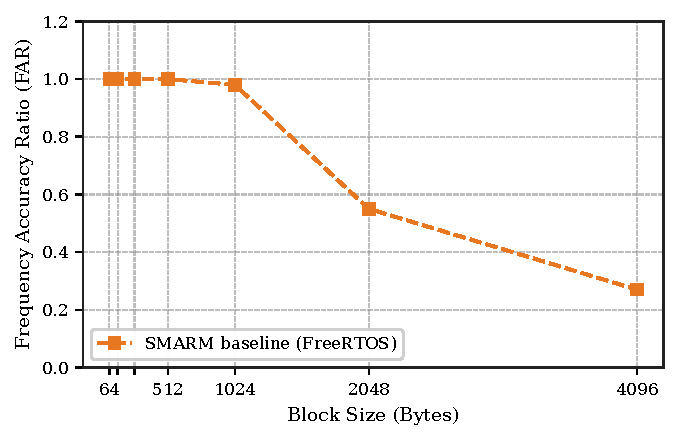
\includegraphics[width=0.7\linewidth]{far_1000.pdf}
        \caption{High real-time workload (1000~Hz)}
        \label{fig:baseline_results_1000hz}
    \end{subfigure}
    \vspace{0.6em}
    \begin{subfigure}[t]{\linewidth}
        \centering
        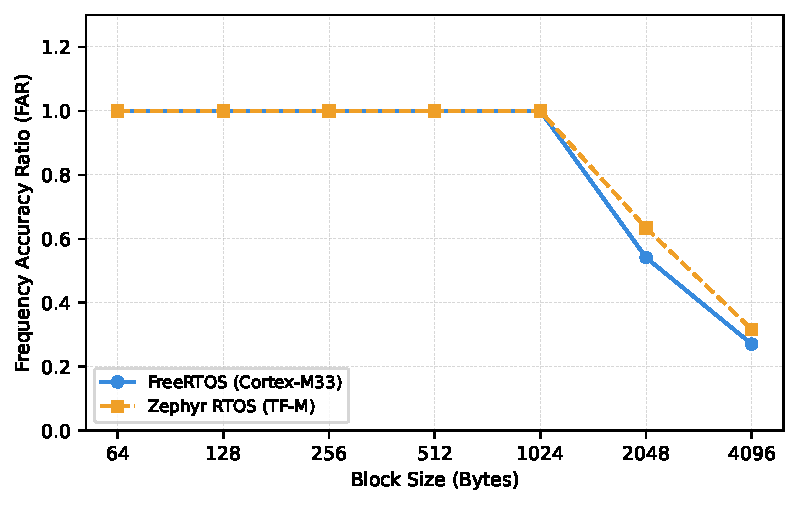
\includegraphics[width=0.7\linewidth]{far_100.pdf}
        \caption{Medium real-time workload (100~Hz)}
        \label{fig:baseline_results_100hz}
    \end{subfigure}
    \vspace{0.6em}
    \begin{subfigure}[t]{\linewidth}
        \centering
        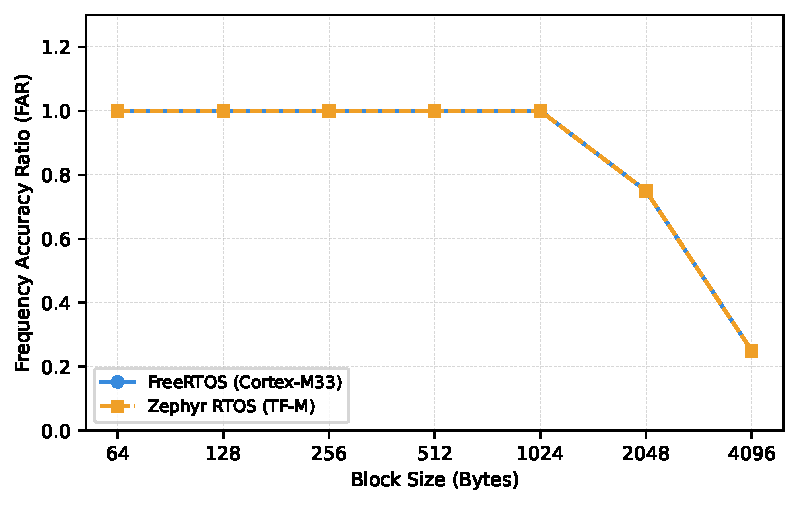
\includegraphics[width=0.7\linewidth]{far_10.pdf}
        \caption{Low real-time workload (10~Hz)}
        \label{fig:baseline_results_10hz}
    \end{subfigure}
    \caption{Real-time availability (FAR) of SMARM under different 
    real-time workloads across block sizes and RTOS platforms. 
    FAR~$\approx 1.0$ for $B \leq 1024$~bytes across all configurations, 
    but degrades significantly at $B \geq 2048$~bytes. Both FreeRTOS and 
    Zephyr exhibit nearly identical trends across all workload classes, 
    indicating that block size rather than RTOS-specific behavior is the 
    dominant factor.}
    \label{fig:setup_and_baseline_far}
\end{figure}
\subsubsection{Interpretation}

The FAR results reveal an important nuance regarding the relationship 
between $t_{\mathrm{disabled}}$ and real-time availability. Although 
$t_{\mathrm{disabled}}$ at $B = 1024$~bytes is already 0.05~ms — 
non-negligible compared to a 1~ms period for a 1000~Hz task — FAR remains 
close to 1.0 at this block size. This is because $T_{RT}$ runs at higher 
priority than the SMARM Wrapper Task and can preempt it between 
consecutive block measurements. The interrupt-disabled window per block is 
short enough that $T_{RT}$ rarely misses a scheduling opportunity. This
observation is independently corroborated by~\cite{joianeto2026iccad},
which reports near-identical timing behavior across FreeRTOS and Zephyr
under TrustZone-M atomic execution on the same Cortex-M33 platform.

However, as $B$ increases beyond 1024~bytes, $t_{\mathrm{disabled}}$ 
grows to the point where $T_{RT}$ begins missing execution slots, causing 
FAR to fall below 1.0. This threshold effect — where FAR is near 1.0 for 
$B \leq 1024$ and then drops sharply — defines the practical boundary of 
SMARM's real-time compatibility on our target platform.

We emphasize that FAR~$\approx 1.0$ is a \textit{necessary} condition for 
real-time compatibility, not a sufficient one. A complete schedulability 
analysis including deadline miss rate, worst-case execution time (WCET), 
and response time is orthogonal to our current study and is left for future 
work. Nevertheless, significant FAR deviation from 1.0 indicates that no 
scheduling policy can guarantee timely task execution in the presence of 
SMARM, making FAR a practically useful indicator.


\subsection{The Storage--Real-Time Trade-off}
\label{sec:storage-tension}

The results above establish that maintaining FAR~$\approx 1.0$ 
requires $B \leq 1024$~bytes on our target platform. We now examine the
opposing constraint --- secure-storage overhead --- and show that it
pulls in the opposite direction as $B$ varies.

SMARM stores the shuffled permutation
$\sigma = \{\sigma(1), \ldots, \sigma(n)\}$ in Secure RAM, where
$n = |M| / B$ is the number of memory blocks. The storage requirement is:
\begin{equation}
    |\sigma| = n \cdot \lceil \log_2 n \rceil \text{ bits}.
    \label{eq:storage}
\end{equation}
As $B$ decreases, $n$ grows inversely, and $|\sigma|$ grows as
$O(n \log n)$. Table~\ref{tab:storage-tradeoff} quantifies this growth
for our target memory size $|M| = 512$~KB.

\begin{table}[H]
    \centering
    \caption{Block size versus secure-storage requirement and
    non-interruptibility period for $|M| = 512$~KB on the STM32L552ZE.
    The shaded row marks the real-time boundary $B = 1024$ bytes, below
    which FAR~$\approx 1.0$.}
    \label{tab:storage-tradeoff}
    \begin{tabular}{rrrr}
        \toprule
        \textbf{Block Size $B$ (bytes)} & \textbf{\# Blocks $n$} &
        \textbf{Secure Storage $|\sigma|$} &
        \textbf{$t_{\text{disabled}}$ (ms)} \\
        \midrule
        64    & 8{,}192 & 13.0~KB  & 0.062 \\
        128   & 4{,}096 & 6.0~KB   & 0.120 \\
        256   & 2{,}048 & 2.75~KB  & 0.237 \\
        512   & 1{,}024 & 1.25~KB  & 0.472 \\
        \rowcolor{gray!15}
        1024  & 512     & 576~B    & 0.939 \\
        2048  & 256     & 256~B    & 1.877 \\
        4096  & 128     & 112~B    & 3.749 \\
        \bottomrule
    \end{tabular}
\end{table}

Table~\ref{tab:storage-tradeoff} reveals the core problem. At 
the real-time boundary of $B = 1024$~bytes, $|\sigma| = 576$~bytes — 
manageable within Secure RAM. However, to preserve FAR across all workload 
levels including high-frequency tasks, even smaller block sizes may be 
preferable. At $B = 256$~bytes, $|\sigma|$ grows to 1.25~KB; at $B = 
64$~bytes, it reaches approximately 13~KB.

On our target platform, the Secure world is allocated 128~KB of SRAM. 
This memory must be shared among all security-critical services co-resident 
in the Secure world, including attestation key storage~\cite{silabs2020an1271}, 
RTOS-aware control-flow integrity monitoring~\cite{kawada2021tzmcfi}, and 
confidential deep-learning inference~\cite{islam2023confidential}. 
Dedicating 10\% or more of Secure RAM solely to the permutation array can 
therefore render SMARM impractical in multi-service deployments, even when 
real-time requirements are otherwise satisfied.

The region of block sizes that satisfy real-time requirements 
($B \leq 1024$~bytes, FAR~$\approx 1.0$) corresponds precisely to the 
region of highest storage overhead under SMARM. Conversely, block sizes 
with manageable storage requirements ($B > 1024$~bytes) violate real-time 
availability. No block size simultaneously achieves both 
FAR~$\approx 1.0$ and acceptable storage overhead under SMARM.

This storage--real-time trade-off is a fundamental limitation of SMARM's 
design: it arises from the requirement to store the full permutation 
$\sigma$ explicitly in Secure RAM, whose size scales as $O(n \log n)$ and 
increases without bound as $B$ decreases. This limitation cannot be resolved by 
block size selection alone, since any choice involves sacrificing either 
real-time availability or storage efficiency.

This finding motivates two complementary contributions in the following 
chapters. In Chapter~\ref{ch:atomic-copy}, we address the real-time dimension by proposing 
the atomic copy enhancement, which reduces $t_{\mathrm{disabled}}$ per 
block from the hash computation time to the much shorter memory copy time, 
thereby extending the range of block sizes for which FAR~$\approx 1.0$ 
can be achieved. In Chapter~\ref{ch:smarmplus}, we address the storage dimension by 
proposing SMARM+, a family of variants that reduce $|\sigma|$ from 
$O(n \log n)$ to $O(n)$ and $O(1)$ without altering real-time behavior, 
enabling deployment on platforms with highly constrained Secure RAM.


\section{Atomic Copy Enhancement and Its Implications}
\label{ch:atomic-copy}

This chapter presents the atomic copy enhancement to SMARM, our third 
contribution. We begin by motivating the need for further reducing the 
non-interruptible window beyond what SMARM achieves. We then describe the 
design and security argument of the enhancement, followed by a comprehensive 
experimental evaluation. Finally, we identify a new practical bottleneck 
revealed by our results — the secure-storage overhead — which motivates the 
SMARM+ variants presented in Chapter~\ref{ch:smarmplus}.


\subsection{Motivation}

As established in Chapter~\ref{ch:eval-smarm}, our TrustZone-M-based 
realization of SMARM successfully reduces the non-interruptibility 
period from the full attestation duration to a single block 
measurement. However, our evaluation on the STM32L552ZE platform 
reveals that this relaxation is insufficient for high-frequency 
real-time workloads: FAR remains close to $1.0$ only when the block 
size $B \leq 1024$~bytes. At larger block sizes (e.g., $B = 4096$ 
bytes), the SHA-256 hash computation per block takes approximately 
$3.75$~ms, which exceeds the period of a 1000~Hz real-time task and 
causes measurable FAR degradation..

The root cause is that SMARM disables interrupts for the entire 
duration of the cryptographic hash computation over each block. 
On our target platform, SHA-256 processes memory at a rate 
(\emph{throughput}) of approximately $1.1$~MB/s, derived 
empirically by measuring $t_{\mathrm{disabled}}$ across block sizes 
and applying $\mathrm{throughput} = B / t_{\mathrm{disabled}}$. As shown in Chapter~\ref{sec:smarm-noninterrupt}, 
$t_{\mathrm{disabled}}$ scales linearly with $B$:
\[
t_{\mathrm{disabled}}^{\text{hash}}(B) \approx \frac{B}{1.1\,\text{MB/s}}.
\]
This means doubling $B$ doubles the interrupt-disabled window, 
directly degrading real-time availability. A key observation is that the hash computation itself does not 
fundamentally need to execute atomically. What must be atomic is 
the \emph{capture} of the memory block: if interrupts were enabled 
during hashing, malware could modify the block's contents after the 
hash begins reading but before it completes, invalidating the 
measurement. However, if a snapshot of the block is first captured 
atomically into a Secure-world buffer, hashing can subsequently 
proceed on that snapshot with interrupts enabled. Since memory copy 
operations are substantially faster than cryptographic hashing 
(typically $15$--$20\times$ on Cortex-M devices), this approach 
significantly shortens the non-interruptibility window while 
preserving measurement correctness.


\subsection{Design: Atomic Copy Protocol}

\subsubsection{Key Insight}

We propose to redesign SMARM's Secure Service such that interrupts 
are disabled only during the memory copy of each block into a 
Secure-world buffer, rather than during the hash computation. After 
the copy completes, interrupts are immediately re-enabled, and the 
hash computation proceeds on the copied data with interrupts on.

This design maintains the security invariant required by SMARM: 
the captured snapshot is guaranteed to faithfully reflect the 
block's state at the moment of capture, since interrupts are 
disabled during the copy operation. Any subsequent modification 
by malware would only affect future captures, not the snapshot 
already taken.

\subsubsection{Protocol Specification}

Algorithm~\ref{alg:enhanced_smarm} details the enhanced SMARM 
protocol with atomic copy.


\begin{algorithm}
\caption{Enhanced SMARM (atomic copy: interrupts disabled around memcpy only)}
\label{alg:enhanced_smarm}
\begin{algorithmic}[1]
\Require $BLOCKS$, $BLOCK\_SIZE$, $indices[0..BLOCKS-1]$, $real\_memory$
\State \Call{HMAC\_Init}{hmac, key}
\For{$i \gets 0$ to $BLOCKS-1$}
  \State $blk \gets$ address of block at $indices[i]\cdot BLOCK\_SIZE$ in $real\_memory$
  \State \Call{DisableInterrupts}{}
  \State \Call{Memcpy}{copy, $blk$, $BLOCK\_SIZE$}
  \State \Call{EnableInterrupts}{}
  \State \Call{HMAC\_Update}{hmac, copy, $BLOCK\_SIZE$}
\EndFor
\State \Call{HMAC\_Finalize}{hmac}
\Ensure digest is available in \textit{hmac.digest}
\end{algorithmic}
\end{algorithm}


The key structural difference from the baseline SMARM 
(Algorithm~\ref{alg:smarm_baseline}) is the separation of each 
block measurement into two distinct operations:

\begin{enumerate}
    \item \textbf{Atomic copy} (interrupts disabled): 
    \texttt{Memcpy(copy, blk, BLOCK\_SIZE)} captures a snapshot 
    of the memory block into a Secure-world buffer.
    \item \textbf{Hash computation} (interrupts enabled): 
    \texttt{HMAC\_Update(hmac, copy, BLOCK\_SIZE)} hashes the 
    captured snapshot.
\end{enumerate}

Since \texttt{Memcpy} operates at memory bandwidth speeds rather 
than cryptographic throughput, the interrupt-disabled window per 
block is reduced from $t_{\mathrm{disabled}}^{\text{hash}}$ to 
$t_{\mathrm{disabled}}^{\text{copy}}$, where 
$t_{\mathrm{disabled}}^{\text{copy}} \ll 
t_{\mathrm{disabled}}^{\text{hash}}$.

\subsubsection{Workflow}
\label{sec:atomic-copy-workflow}


\begin{figure}[H]
    \centering
    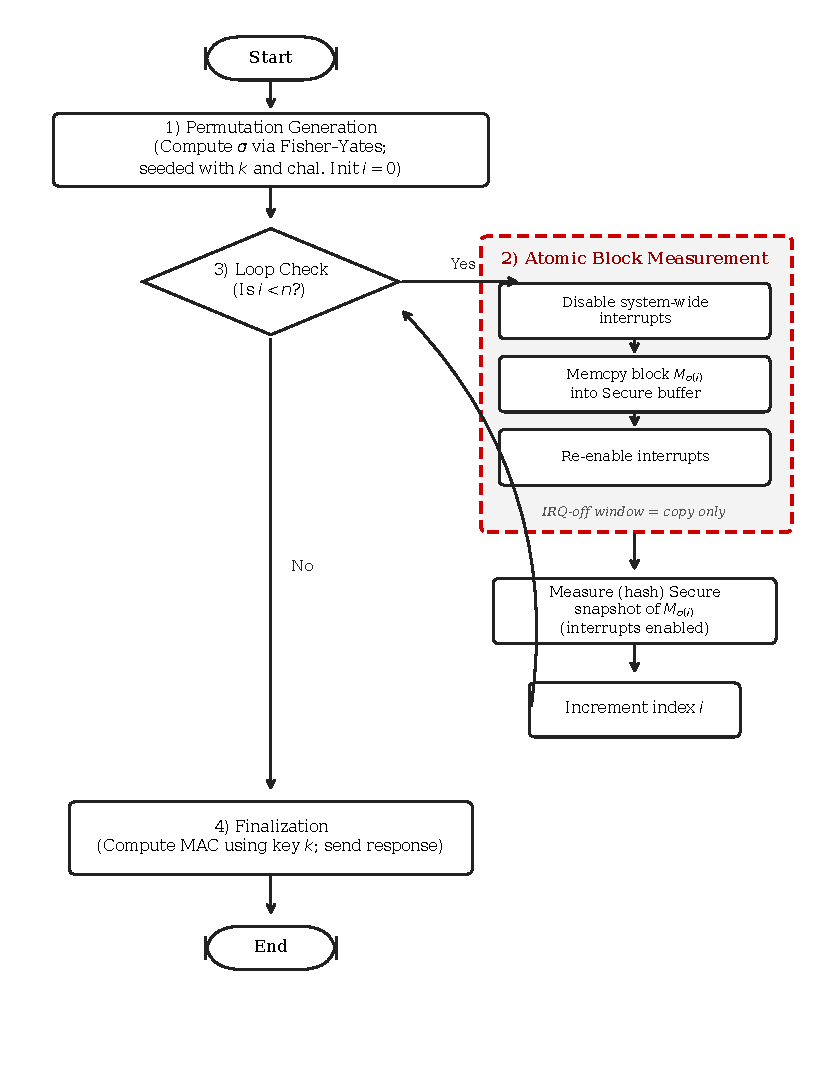
\includegraphics[width=0.85\linewidth]{atomic_workflow.pdf}
    \caption{End-to-end workflow of the atomic copy enhancement. 
    Each iteration consists of two phases: an \emph{atomic copy} step 
    (interrupts disabled) that captures a snapshot of the memory block 
    into a Secure-world buffer, followed by a \emph{hash computation} 
    step (interrupts enabled) over the captured snapshot. Compared to 
    the SMARM baseline (Figure~\ref{fig:smarm_workflow_tz}), the 
    interrupt-disabled window per block is reduced from 
    $t^{\mathrm{hash}}_{\mathrm{disabled}}$ to 
    $t^{\mathrm{copy}}_{\mathrm{disabled}}$, where 
    $t^{\mathrm{copy}}_{\mathrm{disabled}} \ll 
    t^{\mathrm{hash}}_{\mathrm{disabled}}$.}
    \label{fig:atomic_copy_workflow}
\end{figure}

Figure~\ref{fig:atomic_copy_workflow} illustrates the end-to-end 
workflow of the enhanced SMARM Secure Service, which preserves 
the four-phase structure of the SMARM baseline 
(Figure~\ref{fig:smarm_workflow_4phases}). The key difference 
lies in Phase~2, where the atomic operation is shifted from 
hashing to memory copy.

\textbf{Phase 1: Permutation Generation.}
The Secure Service computes the permutation $\sigma$ over the 
memory block indices $\{0, 1, \ldots, n-1\}$ using the 
Fisher-Yates shuffle, seeded from $\mathsf{Hash}(\mathit{chal}, k)$. 
The permutation is stored in Secure RAM, and the loop counter 
$i$ is initialized to $0$. This phase is identical to the 
SMARM baseline.

\textbf{Phase 2: Atomic Block Measurement (redesigned).}
At iteration $i$, the Secure Service retrieves the block index 
$\sigma(i)$ from Secure RAM and performs two distinct sub-steps:
\begin{itemize}
    \item \emph{Atomic copy (interrupts disabled).} The service 
    disables interrupts via the \texttt{CPSID} instruction, 
    invokes $\mathsf{Memcpy}$ to capture a snapshot of block 
    $M_{\sigma(i)}$ into a Secure-world buffer, and immediately 
    re-enables interrupts. This window corresponds to 
    $t_{\mathrm{disabled}}^{\mathrm{copy}}$ — substantially 
    shorter than the original $t_{\mathrm{disabled}}^{\mathrm{hash}}$.
    
    \item \emph{Hash computation (interrupts enabled).} With 
    interrupts enabled, the service invokes 
    $\mathsf{HMAC.Update}$ on the captured snapshot. Real-time 
    tasks may preempt the Wrapper Task during this longer 
    interrupt-enabled window.
\end{itemize}
After both sub-steps complete, the counter $i$ is incremented, 
and control returns to the loop check.

\textbf{Phase 3: Loop Check.}
The Secure Service checks whether all $n$ blocks have been 
measured (i.e., $i = n$). If not, control returns to Phase~2 
to measure the next block in the shuffled order; otherwise, 
execution proceeds to Phase~4. This phase is identical to the 
SMARM baseline.

\textbf{Phase 4: Finalization.}
After all blocks have been measured, the Secure Service 
finalizes the HMAC computation using the attestation key $k$ 
and returns the attestation evidence to the Wrapper Task, 
which forwards it to the verifier. This phase is identical 
to the SMARM baseline.

\textbf{Key design property.}
The key difference from SMARM baseline lies entirely in Phase~2: 
each iteration now consists of a short atomic copy followed by 
a non-atomic hash, with interrupt-enabled windows opening more 
frequently and for longer durations within each iteration. 
This enables real-time tasks to preempt the Wrapper Task more 
often, even when block sizes are large — restoring 
FAR~$\approx 1.0$ at block sizes that previously caused 
real-time violations under the SMARM baseline.

\subsection{Security Argument}

The atomic copy enhancement preserves the same security properties 
as the original SMARM protocol~\cite{carpent2018smarm}. Specifically, 
we argue that all three security requirements (S1)--(S3) defined in 
Chapter~\ref{ch:literature} continue to hold:

\begin{itemize}
    \item \textbf{(S1) Controlled execution.} The Secure Service 
    remains accessible only via TrustZone-M NSC entry points. 
    Interrupts are disabled during the memory copy to ensure the 
    snapshot is captured atomically, preventing malware from 
    modifying the block between the start and end of the copy. 
    The atomicity requirement is preserved — only the protected 
    operation has shifted from hashing to copying.
    
    \item \textbf{(S2) Key secrecy.} The attestation key $k$ and 
    all HMAC-related state remain exclusively in Secure RAM 
    throughout execution. The atomic copy enhancement does not 
    modify the storage or usage of $k$.
    
    \item \textbf{(S3) Private measurement order.} The shuffled 
    permutation $\sigma$ continues to reside in Secure RAM and is 
    not exposed to the Non-Secure world. The atomic copy 
    enhancement does not alter the permutation generation or 
    storage mechanism.
\end{itemize}

The critical security invariant is that interrupts must remain 
disabled for the entire duration of the memory copy operation. 
If malware could interrupt execution after the copy has begun 
but before it completes, it could modify the source block in 
Non-Secure RAM during the copy, potentially causing the Secure-world 
buffer to capture a partially modified block. Disabling interrupts 
during \texttt{Memcpy} prevents this race condition, ensuring that 
the captured snapshot faithfully reflects the block's state at the 
moment the copy began. Subsequent hash computation operates 
exclusively on this protected snapshot in Secure RAM, which is 
inaccessible to Non-Secure malware regardless of interrupt state.


\subsection{Experimental Evaluation}

\subsubsection{Setup}

We evaluate the atomic copy enhancement on the same STM32L552ZE 
development board running FreeRTOS, using the experimental setup 
described in Chapter~\ref{sec:smarm-impl}. We focus our evaluation 
on FreeRTOS since, as established in 
Chapter~\ref{sec:smarm-noninterrupt}, FreeRTOS and Zephyr yield 
nearly identical $t_{\mathrm{disabled}}$ values across all block 
sizes; the conclusions drawn here therefore generalize to Zephyr.

We measure two quantities for each block size 
$B \in \{64, 128, 256, 512, 1024, 2048, 4096\}$~bytes:
\begin{itemize}
     \item The non-interruptibility period 
    $t_{\mathrm{disabled}}^{\text{copy}}$, measured using the 
    on-chip TIM2 hardware timer of the STM32L552ZE. TIM2 is 
    a general-purpose 32-bit timer driven by the system clock; 
    we configure it at $137.5$~kHz (corresponding to a tick 
    resolution of $7.27$~$\mu$s per tick), which provides 
    sufficient precision for measuring sub-millisecond 
    interrupt-disabled windows. Each measurement is averaged 
    over 5 rounds of 5 iterations each.
    
    \item The Frequency Accuracy Ratio (FAR) for three real-time 
    workload classes (high: 1000~Hz, medium: 100~Hz, low: 10~Hz), 
    using the same methodology and 10-round protocol described 
    in Section~\ref{sec:smarm-impl}.
\end{itemize}

\subsubsection{Non-Interruptibility Period}
\label{sec:atomic-tdisabled}

Table~\ref{tab:tdisabled_comparison} reports the measured 
non-interruptibility period $t_{\mathrm{disabled}}$ for both the 
SMARM baseline and the atomic copy enhancement across all block 
sizes. The atomic copy variant achieves a consistent reduction of 
approximately $15$--$16\times$ for $B \geq 128$~bytes, confirming 
that memory copy throughput on the Cortex-M33 substantially 
exceeds SHA-256 hash throughput.

% [TABLE 1]
\begin{table}[h]
\centering
\caption{Non-interruptibility period $t_{\mathrm{disabled}}$ 
comparison between SMARM baseline and atomic copy enhancement 
on STM32L552ZE running FreeRTOS. Measurements averaged over 
5 rounds of 5 iterations each.}
\label{tab:tdisabled_comparison}
\begin{tabular}{rrrrr}
\toprule
& \multicolumn{2}{c}{\textbf{SMARM Baseline}} 
& \multicolumn{2}{c}{\textbf{Atomic Copy}} \\
\cmidrule(lr){2-3} \cmidrule(lr){4-5}
\textbf{$B$ (bytes)} 
& Mean (ms) & Std (ms) 
& Mean (ms) & Std (ms) \\
\midrule
64    & 0.062 & 0.001 & $<$0.007$^\dagger$ & --- \\
128   & 0.120 & 0.001 & 0.008 & 0.001 \\
256   & 0.237 & 0.001 & 0.015 & 0.001 \\
512   & 0.472 & 0.002 & 0.031 & 0.001 \\
1024  & 0.939 & 0.001 & 0.060 & 0.001 \\
2048  & 1.877 & 0.003 & 0.119 & 0.003 \\
4096  & 3.749 & 0.002 & 0.243 & 0.001 \\
\bottomrule
\end{tabular}

\smallskip
\footnotesize
$^\dagger$ At $B = 64$ bytes, the atomic copy completes within a 
single TIM2 tick (7.27~$\mu$s), preventing direct measurement. 
We therefore report the duration as an upper bound 
($< 0.007$~ms) and the corresponding $t_{\mathrm{disabled}}$ 
reduction as a lower bound ($\geq 71\times$ relative to SMARM 
baseline). The true reduction may be substantially larger but 
cannot be quantified with the available hardware timer.
\end{table}

Figure~\ref{fig:tdisabled_comparison} visualizes this comparison 
on a log-log scale. Both curves scale linearly with $B$, but the 
atomic copy curve sits approximately $15$--$16\times$ below the 
baseline curve. This reduction directly translates into more 
frequent and longer interrupt-enabled windows within each 
measurement iteration, enabling real-time tasks to preempt the 
Wrapper Task more effectively.

% [FIG 2]
\begin{figure}[H]
\centering
\includegraphics[width=0.85\linewidth]{tdisabled_copy_vs_baseline.pdf}
\caption{Non-interruptibility period $t_{\mathrm{disabled}}$ of 
the atomic copy enhancement compared to the SMARM baseline across 
block sizes, on the STM32L552ZE platform. The atomic copy variant 
consistently reduces $t_{\mathrm{disabled}}$ by approximately 
$15$--$16\times$ for $B \geq 128$~bytes. Each point is averaged 
over 5 rounds; error bars show standard deviation (smaller than 
marker size).}
\label{fig:tdisabled_comparison}
\end{figure}

\paragraph{Throughput interpretation.}
Both throughput values are derived empirically from the measured 
$t_{\mathrm{disabled}}$ data in Table~\ref{tab:tdisabled_comparison} 
using the relation $\mathrm{throughput} = B / t_{\mathrm{disabled}}$.
Across all block sizes $B \geq 128$~bytes, SHA-256 yields a 
consistent throughput of approximately $1.05$--$1.07$~MB/s 
(reported as $\sim 1.1$~MB/s), while memory copy reaches 
approximately $17$~MB/s — a throughput ratio of $\sim 15.5\times$.

\subsubsection{Real-Time Availability}
\label{sec:atomic-far}

We next evaluate whether the reduction in $t_{\mathrm{disabled}}$ 
translates into improved real-time availability. 
Figure~\ref{fig:far_atomic_copy} presents FAR results for the 
atomic copy enhancement across all block sizes and the three 
real-time workload classes, with SMARM baseline results shown 
for comparison.


\begin{figure}[H]
\centering
\begin{subfigure}[t]{\linewidth}
    \centering
    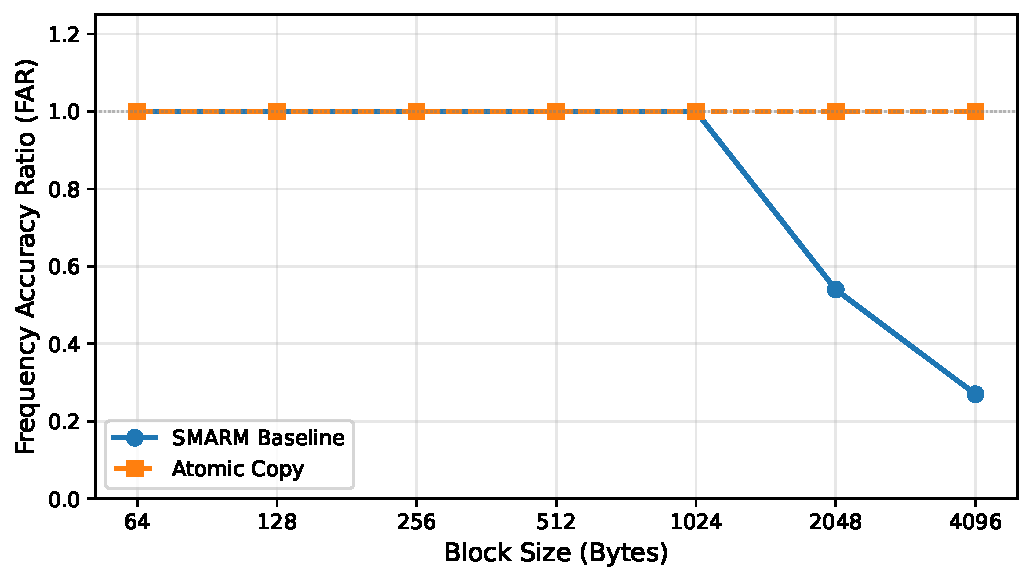
\includegraphics[width=0.7\linewidth]{far_atomic_1000hz.pdf}
    \caption{High real-time workload (1000~Hz)}
    \label{fig:far_atomic_1000}
\end{subfigure}
\vspace{0.5em}
\begin{subfigure}[t]{\linewidth}
    \centering
    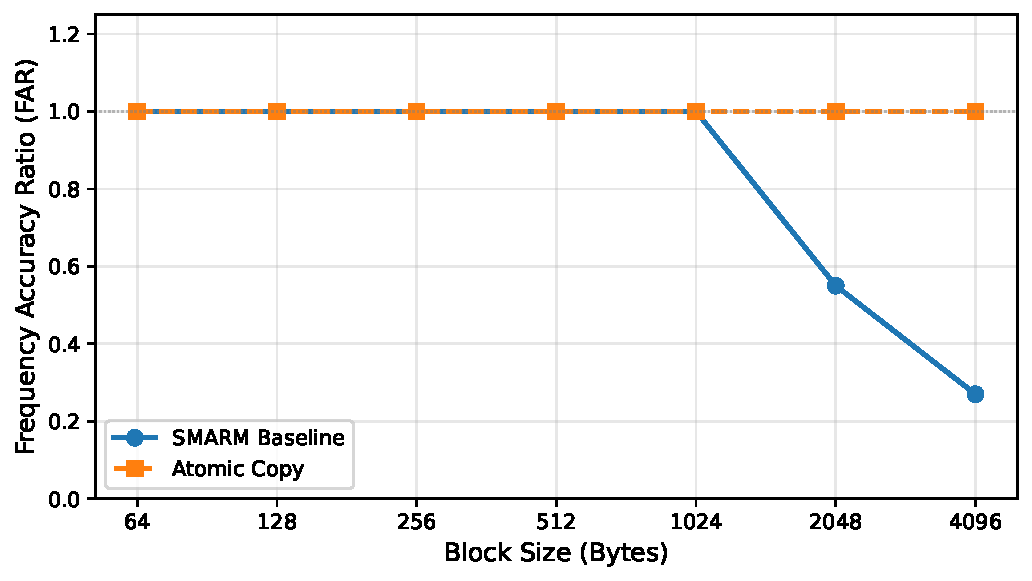
\includegraphics[width=0.7\linewidth]{far_atomic_100hz.pdf}
    \caption{Medium real-time workload (100~Hz)}
    \label{fig:far_atomic_100}
\end{subfigure}
\vspace{0.5em}
\begin{subfigure}[t]{\linewidth}
    \centering
    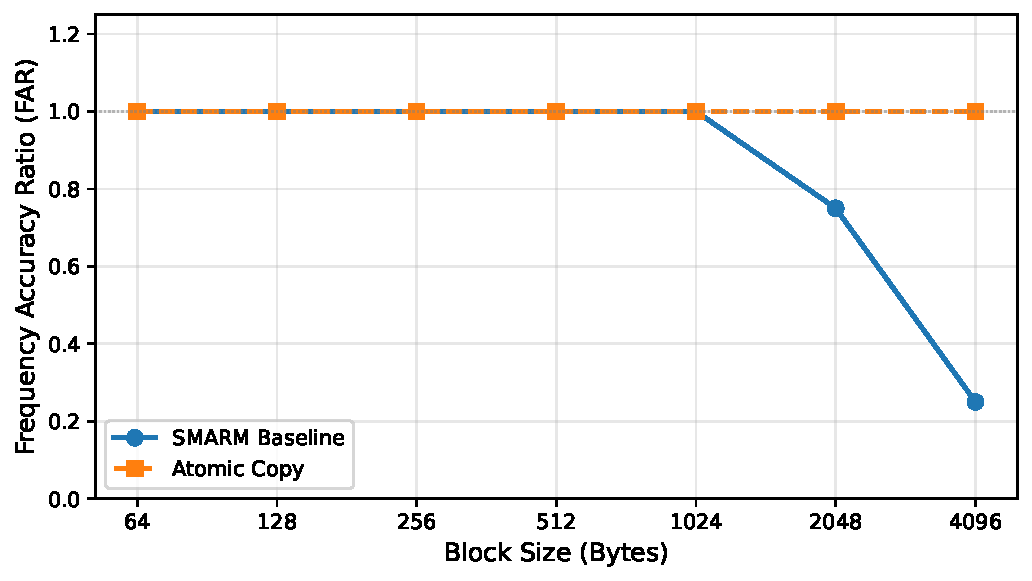
\includegraphics[width=0.7\linewidth]{far_atomic_10hz.pdf}
    \caption{Low real-time workload (10~Hz)}
    \label{fig:far_atomic_10}
\end{subfigure}
\caption{Real-time availability (FAR) of the atomic copy 
enhancement compared to SMARM baseline across block sizes and 
real-time workload classes on STM32L552ZE running FreeRTOS. The 
atomic copy variant maintains FAR~$\approx 1.0$ across all block 
sizes up to 4096 bytes, while the baseline degrades sharply at 
$B \geq 2048$ bytes.}
\label{fig:far_atomic_copy}
\end{figure}

The results reveal a striking improvement: \textbf{the atomic copy 
enhancement maintains FAR~$\approx 1.0$ across all evaluated block 
sizes and all workload classes}, including the previously 
problematic range $B \in \{2048, 4096\}$~bytes. In contrast, the 
SMARM baseline degrades to FAR~$\approx 0.55$ at $B = 2048$~bytes 
and FAR~$\approx 0.27$ at $B = 4096$~bytes under high-frequency 
workloads.

This result has important practical implications. With the atomic 
copy enhancement, designers are no longer constrained to use small 
block sizes to satisfy real-time requirements — any block size 
within the evaluated range becomes viable from a real-time 
perspective. The trade-off boundary shifts from a real-time concern 
to a secure-storage concern, as discussed in 
Section~\ref{sec:atomic-storage-bottleneck}.

\paragraph{Interpretation.}
The improvement in FAR can be understood as follows. Under SMARM 
baseline at $B = 4096$~bytes, each block measurement disables 
interrupts for $3.75$~ms — exceeding the $1$~ms period of a 
1000~Hz real-time task by nearly $4\times$. This means $T_{RT}$ 
cannot execute its required $2$--$3$ iterations during each block 
measurement window, leading to the observed FAR degradation 
across the 64 block measurements per attestation. Under atomic copy 
at the same block size, the interrupt-disabled window per block 
shrinks to only $0.24$~ms — well below the 1~ms task period — 
allowing the task to preempt within the long interrupt-enabled 
hash computation that follows.

\subsection{Implication: The Secure-Storage Bottleneck}
\label{sec:atomic-storage-bottleneck}

The atomic copy enhancement successfully addresses the \emph{real-time} 
dimension of SMARM's coexistence problem: by shifting the atomic 
operation from cryptographic hashing to memory copy, the 
non-interruptibility period $t_{\mathrm{disabled}}$ is reduced by 
$15$--$71\times$ across the evaluated block sizes, and FAR remains 
close to $1.0$ even at the largest block sizes that previously caused 
real-time violations under the SMARM baseline.

However, this improvement does not address the separate 
\emph{secure-storage} dimension of the trade-off identified in 
Section~\ref{sec:storage-tension}. Because the atomic copy enhancement 
does not modify how the permutation $\sigma$ is generated or stored, 
the permutation storage requirement remains 
$|\sigma| = n \cdot \lceil \log_2 n \rceil$ bits, growing 
in the wrong direction as the block size decreases. Furthermore, 
atomic copy itself introduces an additional Secure-RAM requirement: 
a Secure-world buffer of size $B$ bytes is needed to hold the 
captured snapshot during each block measurement. The total 
secure-storage requirement therefore becomes:
\begin{equation}
    \text{Total storage} = \underbrace{n \cdot \lceil \log_2 n \rceil 
    \text{ bits}}_{\text{permutation } \sigma} 
    + \underbrace{B \text{ bytes}}_{\text{atomic copy buffer}}.
\end{equation}
While the buffer is $O(B)$ rather than $O(n \log n)$, it 
compounds the storage cost when small block sizes are used.

In fact, the atomic copy enhancement changes — rather than 
resolves — the underlying problem. Under SMARM baseline, designers 
were naturally limited to use larger block sizes 
($B \leq 1024$~bytes) to maintain FAR~$\approx 1.0$, which 
as a side effect kept the permutation storage moderate (at most 576 
bytes on our target platform). With atomic copy, real-time 
compatibility is preserved even at smaller block sizes, making such 
configurations potentially attractive for security reasons — 
smaller blocks reduce the granularity at which malware can hide 
between measurements, increasing SMARM's detection probability. 
However, these configurations demand much larger Secure RAM 
allocations: up to approximately $13$~KB at $B = 64$~bytes (see 
Table~\ref{tab:storage-tradeoff}).

On TrustZone-M devices, Secure RAM is strictly limited and must 
typically be shared with other security-critical services such as 
confidential deep-learning inference~\cite{islam2023confidential}, 
RTOS-aware control-flow integrity 
monitoring~\cite{kawada2021tzmcfi}, and secure key 
storage~\cite{silabs2020an1271}.Dedicating $10\%$ or more of 
Secure RAM solely to the permutation array can make SMARM 
impractical in multi-service deployments, even when real-time 
requirements are otherwise satisfied.

This observation shows that the atomic copy enhancement, while 
necessary for real-time compatibility, is not sufficient on its 
own to enable practical deployment of SMARM on highly 
resource-constrained platforms. An additional mechanism is 
needed to reduce the secure-storage overhead $|\sigma|$ without 
sacrificing the real-time gains established in this chapter. We 
address this remaining bottleneck in 
Chapter~\ref{ch:smarmplus} by proposing SMARM+, a family of 
storage-efficient SMARM variants that preserve both the security 
guarantees and the real-time behavior established here.


\section{SMARM+: Storage-Efficient Shuffled Attestation}
\label{ch:smarmplus}

This chapter presents SMARM+, our fourth contribution, designed to 
address the secure-storage bottleneck identified in 
Chapter~\ref{ch:atomic-copy}. We propose two complementary variants 
— SMARM+PRNG (based on a Pseudorandom Number 
Generator) and SMARM+FPE(based on Format-Preserving 
Encryption) — that reduce the secure-storage requirement from 
$O(n \log n)$ bits to $O(n)$ and $O(1)$ bits respectively, while 
preserving both the security guarantees of SMARM and the real-time 
behavior established by the atomic copy enhancement.

\subsection{Motivation}
\label{sec:smarmplus-motivation}

The atomic copy enhancement of Chapter~\ref{ch:atomic-copy} 
successfully addresses the real-time dimension of SMARM's coexistence 
problem: FAR remains close to $1.0$ across all evaluated block sizes 
(64--4096 bytes). However, this real-time improvement does not 
address the separate \emph{secure-storage} dimension of the 
trade-off. As established in Chapter~\ref{sec:storage-tension} and
quantified in Table~\ref{tab:storage-tradeoff}, the permutation 
$\sigma$ requires $|\sigma| = n \cdot \lceil \log_2 n \rceil$ bits 
of Secure RAM, growing in the wrong direction as block size $B$ 
decreases and becoming too costly on TrustZone-M devices where 
Secure RAM must be shared with other security-critical 
services~\cite{islam2023confidential, kawada2021tzmcfi, silabs2020an1271}.

Even when designers try to handle this issue by selecting 
larger block sizes ($B \geq 2048$ bytes) to reduce $|\sigma|$, two 
constraints arise. First, although the atomic copy enhancement 
makes large block sizes real-time compatible, the security 
analysis of SMARM~\cite{carpent2018smarm} shows that smaller 
block sizes provide a higher detection probability against roving 
malware, since they reduce the granularity at which malware can 
hide between measurements. Second, in highly constrained 
deployments, even the $|\sigma|$ at $B = 4096$ bytes (112 bytes) 
may not be acceptable if Secure RAM is heavily shared by other 
services. Both factors motivate a basic redesign of how 
SMARM stores its permutation state.

The key insight underlying SMARM+ is that the permutation $\sigma$ 
need not be stored as an explicit array in Secure RAM. 
What SMARM actually requires from $\sigma$ is two properties:

\begin{enumerate}
    \item \textbf{Coverage}: every block must be measured exactly once.
    \item \textbf{Unpredictability}: the next block to measure must 
    not be predictable by KFV malware.
\end{enumerate}

If both properties can be satisfied by an alternative representation 
that uses less secure memory, the storage bottleneck can be 
eliminated without sacrificing security. SMARM+ achieves this 
through two design strategies, presented in the following 
sections.


\subsection{Design Approach}
\label{sec:smarmplus-design}

\subsubsection{Trading Storage for Computation}

SMARM+ keeps the same high-level architecture as 
SMARM~\cite{carpent2018smarm}, consisting of a Non-Secure Wrapper 
Task and a Secure Service. The Wrapper Task is unchanged. Only the 
Secure Service is redesigned to compute the measurement order 
at runtime during each attestation, rather than storing it 
in advance.

This redesign reflects a basic trade-off: \textbf{reducing 
secure storage requires additional computation per iteration}. In 
the baseline SMARM, the permutation is generated once via 
Fisher-Yates and stored explicitly; subsequent block lookups take 
$O(1)$ time. In SMARM+, the next block index is computed 
dynamically at each iteration, adding a per-block cost in 
exchange for reduced secure-storage footprint.

\subsubsection{Two-Variant Strategy}

We propose two variants that sit at different points on the 
storage-vs-computation trade-off curve:

\begin{itemize}
    \item \textbf{SMARM+PRNG} 
    (Chapter~\ref{sec:smarmplus-prng}) replaces the explicit 
    permutation array with a small $n$-bit bitmap that tracks 
    which blocks have already been measured. Storage drops from 
    $O(n \log n)$ to $O(n)$ bits.
    
    \item \textbf{SMARM+FPE} 
    (Chapter~\ref{sec:smarmplus-fpe}) eliminates per-block 
    permutation state entirely by deriving the measurement order 
    from a format-preserving 
    encryption~\cite{bellare2009fpe,dworkin2016sp800}. Storage 
    drops to $O(1)$, independent of $n$.
\end{itemize}

Each variant keeps the security guarantees of SMARM (S1)--(S3) 
and the real-time behavior established in Chapter~\ref{ch:atomic-copy}. 
The choice between them depends on the specific Secure-RAM 
constraints of the target platform, as discussed in 
Chapter~\ref{sec:smarmplus-deployment}.

\subsection{SMARM+PRNG: Reducing Storage to $O(n)$}
\label{sec:smarmplus-prng}

\subsubsection{Background: Pseudorandom Number Generators}

SMARM+PRNG reduces secure storage by replacing 
the explicit permutation $\sigma$ with a Pseudorandom Number 
Generator (PRNG) — a deterministic algorithm that, given a 
secret seed, produces a sequence of values that look 
indistinguishable from true random numbers to any party without 
knowledge of the seed. A PRNG has two properties relevant to 
our design:

\begin{itemize}
    \item \textbf{Determinism}: the same seed always produces 
    the same output sequence, allowing the verifier to 
    independently reproduce the measurement order using the 
    shared key and challenge.
    
    \item \textbf{Unpredictability}: without knowledge of the 
    seed, the next output cannot be predicted by KFV malware.
\end{itemize}

In our implementation, we build the PRNG using a 
cryptographic hash function (SHA-256) seeded by 
$\mathsf{Hash}(\mathit{chal}, k)$, where $\mathit{chal}$ is 
the verifier's challenge and $k$ is the attestation key. This 
construction is widely used and gets its security properties 
from the underlying hash function.

The key advantage of using a PRNG over storing $\sigma$ 
explicitly is that the PRNG state can be regenerated 
on-the-fly from the seed during each attestation, requiring 
no persistent storage beyond the key material already used by 
SMARM. However, since the PRNG produces independent random 
values rather than a permutation, an additional mechanism is 
needed to ensure that every block is measured exactly once. 
SMARM+PRNG handles this by maintaining a 
small bitmap that tracks which blocks have already been 
measured, as detailed in the protocol below.


\subsubsection{Protocol}

Instead of storing the full permutation $\sigma$, 
SMARM+PRNG maintains a bitmap \texttt{used} of $n$ 
bits, where \texttt{used}[$i$] indicates whether block $M_i$ has 
already been measured. At each iteration, the algorithm generates 
a random integer $r$ using a PRNG seeded from $k$ and \textit{chal}, 
then scans the bitmap to find the $r$-th unmeasured block. The 
selected block is measured atomically, then marked as measured. 
This process repeats until all $n$ blocks are covered. The full 
procedure is given in Algorithm~\ref{alg:smarmprng}.


\begin{algorithm}
\caption{SMARM+PRNG Secure Service}
\label{alg:smarmprng}
\begin{algorithmic}[1]
\Require Memory $M$, block size $B$, number of blocks $n$, 
         key $k$, challenge \textit{chal}
\For{all $i \in \{0, \ldots, n-1\}$}
    \State $\texttt{used}[i] \gets 0$
\EndFor
\State $\mathit{seed} \gets \Call{Hash}{\mathit{chal}, k}$
\State $\Call{PRNG.Init}{\mathit{seed}}$
\State $\Call{HMAC.Init}{k}$
\For{$r \gets 0$ to $n - 1$}
    \State $\mathit{rem} \gets n - r$
    \State $k' \gets \Call{PRNG.RandInt}{1, \mathit{rem}}$
    \State $\mathit{idx} \gets \Call{FindKthZero}{\texttt{used}, k'}$
    \State $\texttt{used}[\mathit{idx}] \gets 1$
    \State \Call{DisableInterrupts}{}
    \State $\Call{HMAC.Update}{\mathit{hmac}, M_{\mathit{idx}}, B}$
    \State \Call{EnableInterrupts}{}
\EndFor
\State \textbf{return} $\Call{HMAC.Finalize}{\mathit{hmac}}$
\end{algorithmic}
\end{algorithm}

The algorithm proceeds as follows:

\begin{itemize}
    \item \textbf{Lines 1--6 (Initialization).} The \texttt{used} 
    bitmap is initialized to all zeros, indicating that no blocks 
    have been measured. A PRNG is seeded using a hash of the 
    verifier's challenge \textit{chal} and the secret key $k$, 
    ensuring that the random sequence is both fresh and private 
    for each attestation instance.
    
    \item \textbf{Lines 8--11 (Block Selection).} At iteration $r$, 
    the algorithm computes the number of remaining unmeasured 
    blocks ($\mathit{rem}$). It then generates a random 
    integer $k' \in [1, \mathit{rem}]$ and scans the bitmap to 
    locate the $k'$-th zero entry, whose position becomes the 
    block index $\mathit{idx}$. The selected block is marked as 
    measured by setting $\texttt{used}[\mathit{idx}] \gets 1$.
    
    \item \textbf{Lines 12--14 (Atomic Measurement).} The block 
    $M_{\mathit{idx}}$ is measured atomically using the same 
    interrupt-disable/enable pattern as SMARM. This step can 
    also use the atomic copy enhancement from 
    Chapter~\ref{ch:atomic-copy} to further reduce 
    $t_{\mathrm{disabled}}$.
\end{itemize}

\subsubsection{Workflow}
\label{sec:smarmprng-workflow}

Figure~\ref{fig:smarmprng_workflow} illustrates the end-to-end 
workflow of SMARM+PRNG. The workflow consists 
of five phases, with a clear Block Selection phase that 
replaces the hidden permutation lookup of SMARM. Compared 
to the baseline (Figure~\ref{fig:smarm_workflow_4phases}), the 
additional phase makes the per-block bitmap scan overhead 
visible.

\begin{figure}[H]
\centering
\includegraphics[width=0.95\linewidth]{smarmprng_workflow.pdf}
\caption{End-to-end workflow of SMARM+PRNG. 
The block selection phase (blue dashed box) runs with 
interrupts enabled, while only the HMAC update over the 
selected block (red dashed box) requires interrupts to be 
disabled. The \texttt{used} bitmap tracks which blocks have 
been measured, replacing the explicit permutation array of 
SMARM.}
\label{fig:smarmprng_workflow}
\end{figure}

\textbf{Phase 1: Initialization.}
The Secure Service initializes the \texttt{used} bitmap to all 
zeros, indicating that no blocks have been measured. It then 
seeds the PRNG using $\mathsf{Hash}(\mathit{chal}, k)$, ensuring 
that the random sequence is both fresh (depending on the 
verifier's challenge) and private (depending on the secret 
key~$k$). The loop counter $r$ is initialized to $0$.

\textbf{Phase 2: Block Selection (interrupts enabled).}
The service computes $k' \gets \mathsf{PRNG.RandInt}(1, n-r)$ 
where $n - r$ is the number of remaining unmeasured blocks. 
It then scans the \texttt{used} bitmap via 
$\mathsf{FindKthZero}$ to find the $k'$-th zero entry, 
whose position becomes the next block index 
$\mathit{idx}$. Finally, $\mathit{idx}$ is marked as 
measured by setting $\texttt{used}[\mathit{idx}] \gets 1$. 
All operations in this phase run with interrupts 
enabled, allowing real-time tasks to preempt the Wrapper 
Task during the $O(n)$ bitmap scan. This phase is 
the main computational overhead added by 
SMARM+PRNG compared to the SMARM baseline.

\textbf{Phase 3: Atomic Block Measurement (interrupts disabled).}
The service disables interrupts via the 
\texttt{CPSID} instruction, calls 
$\mathsf{HMAC.Update}(\mathit{hmac}, M_{\mathit{idx}}, B)$ 
to add the selected block into the running hash, 
and immediately re-enables interrupts. This atomic window 
has the same duration as the SMARM baseline, 
keeping $t_{\mathrm{disabled}}$ and therefore the FAR 
behavior established in Chapter~\ref{ch:eval-smarm}.

After completing Phase 3, the counter $r$ is incremented, 
and control returns to the loop check.

\textbf{Phase 4: Loop Check.}
The Secure Service checks whether all $n$ blocks have been 
measured (i.e., $r = n$). If not, control returns to Phase~2 
to select the next block; otherwise, execution proceeds to 
Phase~5.

\textbf{Phase 5: Finalization.}
Once all $n$ blocks have been measured, the Secure Service 
finalizes the HMAC computation using the attestation key $k$, 
producing the attestation evidence. This evidence is returned 
to the Wrapper Task, which forwards it to the verifier.

\textbf{Key design property.}
An important point of this workflow is that the additional 
computation added by SMARM+PRNG 
(\textsf{PRNG.RandInt}, \textsf{FindKthZero}, and bitmap update) 
runs \emph{outside} the atomic critical section. This 
ensures that the new mechanism does not extend the 
non-interruptibility period~$t_{\mathrm{disabled}}$ compared to 
SMARM. The added overhead shows up in overall attestation 
runtime, not in real-time interference — a property we verify 
through experiments in Chapter~\ref{sec:smarmplus-eval}.

\subsubsection{Soundness Argument}

We argue that SMARM+PRNG is functionally equivalent 
to SMARM by showing that (1) all memory blocks are measured exactly 
once, and (2) the order of block selection is uniformly random.

\textbf{Coverage.} At each iteration, the algorithm selects an 
index $\mathit{idx}$ such that $\texttt{used}[\mathit{idx}] = 0$, 
then sets it to $1$. Since each iteration flips exactly one bit 
from $0$ to $1$, and there are $n$ such bits, after $n$ iterations 
all entries in \texttt{used} are set to $1$. This guarantees that 
every block is selected exactly once.

\textbf{Randomness.} The PRNG is seeded from a secret key $k$, 
making its outputs unpredictable to any party without knowledge 
of $k$. At iteration $r$, the algorithm samples a uniform random 
integer $k' \in [1, \mathit{rem}]$. The mapping from $k'$ to the 
$k'$-th zero entry in \texttt{used} establishes a one-to-one 
correspondence between $k'$ and the set of remaining unmeasured 
blocks. Therefore, each unmeasured block is selected with equal 
probability at each step, and the overall measurement order is a 
uniformly random permutation over all $n$ blocks.

\subsubsection{Security Argument}

We argue that SMARM+PRNG retains the same security 
guarantees as SMARM by meeting all three requirements 
(S1)--(S3) defined in Chapter~\ref{ch:literature}:

\begin{itemize}
    \item \textbf{(S1) Controlled execution.} 
    SMARM+PRNG preserves both design choices of 
    SMARM for enforcing (S1): it implements its logic as a 
    Secure-world service accessible only via TrustZone-M NSC 
    entry points, and it disables interrupts during each block 
    measurement to ensure atomic execution. Therefore, (S1) is 
    directly preserved.
    
    \item \textbf{(S2) Key secrecy.} 
    SMARM+PRNG does not modify the generation, 
    storage, or usage of the attestation key $k$. As in SMARM, 
    $k$ is stored and accessed exclusively within Secure RAM.
    
    \item \textbf{(S3) Private measurement order.} 
    In SMARM+PRNG, the measurement order is 
    implicitly determined by the \texttt{used} bitmap, which 
    resides in Secure RAM inaccessible to the Non-Secure world. 
    
    \emph{Side-channel consideration.} While direct memory 
    access is prevented by TrustZone-M, KFV malware might attempt 
    to infer the measurement order via timing side channels — 
    specifically by observing variations in the duration of 
    \textsc{FindKthZero}. To mitigate this, we implement 
    \textsc{FindKthZero} such that it always scans all $n$ 
    entries of the \texttt{used} bitmap, rather than terminating 
    early upon finding the $k'$-th zero. As a result, its 
    execution time is independent of the selected $\mathit{idx}$, 
    ensuring that the block measurement procedure does not leak 
    information about the measurement order through timing.
    
    Replay attacks are mitigated in the same way as in SMARM: 
    the block order depends on a one-time challenge \textit{chal} 
    and the secret key $k$.
\end{itemize}

\subsubsection{Storage vs Runtime Trade-off}

Compared to SMARM, SMARM+PRNG replaces the explicit 
storage of $\sigma$ with the \texttt{used} bitmap. The storage 
requirement is exactly $n$ bits, reducing the complexity from 
$O(n \log n)$ in SMARM to $O(n)$.

This reduction comes at the cost of additional runtime overhead. 
In SMARM, each block index can be retrieved in $O(1)$ time from 
the pre-computed $\sigma$. In SMARM+PRNG, the 
\textsc{FindKthZero} operation must scan up to $O(n)$ entries 
of the bitmap per iteration. The cumulative cost across all $n$ 
iterations is therefore $O(n^2)$, which can become significant 
when $n$ is large (i.e., when $B$ is small). We quantify this 
overhead empirically in 
Chapter~\ref{sec:smarmplus-runtime-eval}.

\subsection{SMARM+FPE: Eliminating Storage to $O(1)$}
\label{sec:smarmplus-fpe}

\subsubsection{Background: Format-Preserving Encryption}

SMARM+FPE eliminates permutation storage by 
leveraging a cryptographic primitive called Format-Preserving 
Encryption~(FPE)~\cite{bellare2009fpe,dworkin2016sp800}. FPE is a 
symmetric encryption scheme whose ciphertexts share the same domain 
as the plaintexts. Formally, for an encryption key $K \in 
\mathcal{K}$ and a finite domain $\mathcal{D}$, FPE defines:
\[
\textsf{FPE.Enc}: \mathcal{K} \times \mathcal{D} \rightarrow \mathcal{D}
\]

The key property of FPE for our purposes is that for a fixed key, 
$\textsf{FPE.Enc}$ realizes a \emph{bijection} — a one-to-one 
mapping where every element in $\mathcal{D}$ maps to a unique 
element in $\mathcal{D}$, with no collisions. This makes FPE a 
natural instantiation of a pseudo-random permutation~(PRP): given 
the domain $\{0, \ldots, n-1\}$ representing block indices, 
encrypting each $i \in \{0, \ldots, n-1\}$ with the same key 
produces a permutation of the same set.

Standard block ciphers such as AES are not directly suitable here: 
AES operates on fixed 128-bit blocks, so encrypting an integer 
$i \in \{0, \ldots, n-1\}$ with AES would produce a 128-bit 
ciphertext outside the desired domain. FPE precisely addresses 
this mismatch by guaranteeing that the ciphertext remains within 
the same domain as the plaintext, making it directly usable as 
a block index.

\subsubsection{FFX Construction with Speck Cipher}

We instantiate FPE using the FFX 
construction~\cite{bellare2010ffx}, which builds an FPE scheme on 
top of a Feistel network. A Feistel network is a classical 
cipher design that constructs a bijection over a domain by 
iteratively applying a round function based on a standard block 
cipher; the number of rounds determines the security level. FFX 
is widely adopted, standardized by NIST in SP 800-38G~\cite{dworkin2016sp800}, 
and provides provable security under standard cryptographic 
assumptions.

For the underlying block cipher used inside FFX, we choose 
Speck~\cite{beaulieu2015simon} — a lightweight block cipher 
designed by the NSA specifically for constrained software 
environments. Compared to AES, Speck achieves higher throughput 
on Cortex-M devices while requiring a much smaller code 
footprint — approximately 200 bytes of code on ARMv8-M, versus 
several kilobytes for typical AES implementations. This choice 
aligns with our target deployment setting where both runtime 
efficiency and code size are constrained.

\subsubsection{Protocol}

Instead of storing the full permutation $\sigma$ or maintaining 
a per-iteration bitmap as in SMARM+PRNG, SMARM+FPE eliminates 
permutation state entirely by deriving each block index directly 
from FFX encryption. At iteration $i$, the algorithm computes 
the block index as $\mathit{idx} \gets \textsf{FFX.Enc}(i)$, 
where the FFX key and tweak are derived from the attestation 
key $k$ and the verifier's challenge \textit{chal}. Since FFX 
realizes a bijection over $\{0, \ldots, n-1\}$, iterating $i$ 
from $0$ to $n-1$ produces a permutation where every block is 
measured exactly once — without storing any per-iteration state. 
The full procedure is given in Algorithm~\ref{alg:smarmfpe}.

\begin{algorithm}
\caption{SMARM+FPE Secure Service}
\label{alg:smarmfpe}
\begin{algorithmic}[1]
\Require Memory $M$, block size $B$, number of blocks $n$, 
         key $k$, challenge \textit{chal}
\State $(\mathit{ffx\_key}, \mathit{tweak}) \gets 
       \Call{KDF}{k, \mathit{chal}}$
\State $\Call{FFX.Init}{\mathit{ffx\_key}, \mathit{tweak}}$
\State $\Call{HMAC.Init}{k}$
\For{$i \gets 0$ to $n - 1$}
    \State $\mathit{idx} \gets \Call{FFX.Enc}{i}$
    \State \Call{DisableInterrupts}{}
    \State $\Call{HMAC.Update}{\mathit{hmac}, M_{\mathit{idx}}, B}$
    \State \Call{EnableInterrupts}{}
\EndFor
\State \textbf{return} $\Call{HMAC.Finalize}{\mathit{hmac}}$
\end{algorithmic}
\end{algorithm}

The algorithm operates as follows:

\begin{itemize}
    \item \textbf{Lines 1--3 (Initialization).} The FFX key and 
    tweak are derived from the attestation key $k$ and the 
    verifier's challenge \textit{chal} using a key derivation 
    function (KDF). The FFX instance is initialized with these 
    parameters, and HMAC is initialized with the attestation key.
    
    \item \textbf{Lines 4--8 (Block Measurement Loop).} At 
    iteration $i$, the algorithm computes the next block index 
    by encrypting $i$ with FFX: $\mathit{idx} \gets 
    \textsf{FFX.Enc}(i)$. The corresponding block 
    $M_{\mathit{idx}}$ is then measured atomically. Since FFX 
    realizes a bijection over $\{0, \ldots, n-1\}$, iterating 
    $i$ from $0$ to $n-1$ produces a permutation where every 
    block is measured exactly once.
\end{itemize}

\subsubsection{Workflow}
\label{sec:smarmfpe-workflow}

Figure~\ref{fig:smarmfpe_workflow} illustrates the end-to-end 
workflow of SMARM+FPE. Compared to 
SMARM+PRNG 
(Figure~\ref{fig:smarmprng_workflow}), the workflow is 
substantially simplified: the block-selection phase reduces to a 
single FFX encryption, and no per-block state needs to be 
maintained in Secure RAM.

\begin{figure}[H]
\centering
\includegraphics[width=0.95\linewidth]{smarmfpe_workflow.pdf}
\caption{End-to-end workflow of SMARM+FPE. 
The block selection phase (blue dashed box) reduces to a single 
$\mathsf{FFX.Enc}(i)$ call, eliminating the bitmap-tracking 
overhead of SMARM+PRNG. The atomic block 
measurement (red dashed box) is identical to SMARM, preserving 
the same $t_{\mathrm{disabled}}$ and FAR behavior.}
\label{fig:smarmfpe_workflow}
\end{figure}

\textbf{Phase 1: Initialization.}
The Secure Service derives the FFX key and tweak from 
$\mathsf{KDF}(k, \mathit{chal})$, where the KDF (Key Derivation 
Function) is realized using HMAC-SHA256 with $k$ and 
$\mathit{chal}$ as inputs. The FFX instance is initialized with 
these derived parameters via $\mathsf{FFX.Init}$. The loop 
counter $i$ is initialized to $0$.

\textbf{Phase 2: Block Selection (interrupts enabled).}
The service computes the next block index directly via 
$\mathit{idx} \gets \mathsf{FFX.Enc}(i)$. Since FFX realizes 
a bijection over the domain $\{0, \ldots, n-1\}$, iterating 
$i$ from $0$ to $n-1$ produces a uniformly random 
permutation in which every block is selected exactly once 
— without needing any auxiliary tracking structure such as 
the \texttt{used} bitmap in SMARM+PRNG. The 
FFX encryption is performed with interrupts enabled, 
allowing real-time tasks to preempt the Wrapper Task during 
this computation. This phase represents the main computational 
overhead introduced by SMARM+FPE compared to 
the SMARM baseline.

\textbf{Phase 3: Atomic Block Measurement (interrupts disabled).}
As in SMARM+PRNG and the SMARM baseline, the 
service disables interrupts, invokes 
$\mathsf{HMAC.Update}(\mathit{hmac}, M_{\mathit{idx}}, B)$, 
and re-enables interrupts. The atomic window is identical 
to SMARM, preserving FAR behavior.



After completing Phase 3, the counter $i$ is incremented, and 
control returns to the loop check.

\textbf{Phase 4: Loop Check.}
The Secure Service checks whether all $n$ blocks have been 
measured. If not, control returns to Phase~2 to select the next 
block; otherwise, execution proceeds to Phase~5.

\textbf{Phase 5: Finalization.}
After all $n$ blocks have been measured, the Secure Service 
finalizes the HMAC computation and returns the attestation 
evidence to the Wrapper Task, which forwards it to the verifier.

\textbf{Key design property.}
The most significant difference from SMARM+PRNG 
is the absence of any permutation-tracking state. The FFX 
instance maintains only constant-size key material (the FFX key 
and tweak derived in Phase~1), regardless of the number of 
blocks $n$. This eliminates the $O(n)$ Secure-RAM dependence of 
SMARM+PRNG, achieving the $O(1)$ storage 
complexity claimed in 
Section~\ref{sec:smarmplus-fpe}. The trade-off is that each 
$\mathsf{FFX.Enc}$ invocation requires multiple Speck rounds, 
imposing a per-iteration cryptographic cost — analyzed 
empirically in Section~\ref{sec:smarmplus-eval}.

\subsubsection{Soundness Argument}

\textbf{Coverage.} SMARM+FPE iterates over 
$i \in \{0, \ldots, n-1\}$ and maps each $i$ to a block index 
$\mathit{idx} = \textsf{FFX.Enc}(i)$. Since FFX realizes a 
bijection over the domain $\{0, \ldots, n-1\}$, each value of 
$\mathit{idx}$ is distinct for distinct values of $i$. Therefore, 
every block is measured exactly once.

\textbf{Randomness.} The randomness of the measurement order 
follows directly from the pseudo-random permutation property of 
FFX. The order of block selection is precisely 
$\{\textsf{FFX.Enc}(0), \textsf{FFX.Enc}(1), \ldots, 
\textsf{FFX.Enc}(n-1)\}$, which is computationally 
indistinguishable from a uniformly random permutation under the 
assumption that the underlying Speck cipher is a pseudo-random 
function.

\subsubsection{Security Argument}

We argue that SMARM+FPE retains the same security guarantees 
as SMARM by meeting all three requirements (S1)--(S3) defined 
in Chapter~\ref{ch:literature}:

\begin{itemize}
    \item \textbf{(S1) Controlled execution.} 
    SMARM+FPE preserves the design choices of 
    SMARM: the Secure Service is accessible only via TrustZone-M 
    NSC entry points, and interrupts are disabled during each 
    block measurement via the \texttt{CPSID} instruction to 
    ensure atomic execution. Therefore, (S1) is directly preserved.
    
    \item \textbf{(S2) Key secrecy.} 
    SMARM+FPE does not modify the generation, 
    storage, or usage of the attestation key $k$. As in SMARM, 
    $k$ is stored and accessed exclusively within Secure RAM, 
    and is used only to derive the FFX key and tweak — both of 
    which also remain confined to the Secure world.
    
    \item \textbf{(S3) Private measurement order.} The 
    measurement order is determined by \textsf{FFX.Enc}, whose 
    output depends on the FFX key derived from the secret $k$ 
    and the one-time challenge \textit{chal}. Since the FFX key 
    resides exclusively in Secure RAM, KFV malware cannot 
    compute or predict the permutation. 

     \emph{Side-channel consideration.} Unlike SMARM+PRNG, 
    SMARM+FPE does not require a side-channel analysis for 
    \textsf{FFX.Enc}, since the FFX construction performs a 
    fixed number of Feistel rounds regardless of the input, 
    yielding a constant-time computation that does not leak 
    information about $\mathit{idx}$ through timing.
    
    Replay attacks are mitigated in the same way as in SMARM: 
    the FFX key and tweak depend on a one-time challenge 
    \textit{chal} and the secret key $k$.
    
\end{itemize}

\textbf{Small-domain considerations.} A potential concern with 
FFX-based FPE is its known vulnerability to small-domain attacks 
when the adversary can observe or query multiple 
plaintext-ciphertext pairs~\cite{hoang2018curse}. In our setting, 
however, these attack conditions do not arise for two reasons. 
First, SMARM+FPE does not expose the ciphertext 
outputs $\mathit{idx}$ to the Non-Secure world; they remain 
internal to the Secure-world measurement loop. Second, the FFX 
instance does not provide oracle access to untrusted code. As a 
result, malware cannot accumulate the plaintext-ciphertext pairs 
required to mount small-domain attacks. Hardening SMARM+FPE against side-channel leakage of these 
internal values is left as future work.

\subsubsection{Storage vs Runtime Trade-off}

Compared to both SMARM and SMARM+PRNG, SMARM+FPE eliminates 
per-block permutation state entirely. The only secure-storage 
requirements are the FFX key and the HMAC state, both of which 
are $O(1)$ in size and independent of $n$. On our platform, this 
corresponds to a fixed overhead of approximately $16$ bytes for 
FFX key material, reducing the storage complexity from 
$O(n \log n)$ in SMARM and $O(n)$ in SMARM+PRNG to $O(1)$.

This elimination comes at the cost of additional per-block 
cryptographic computation. While the FFX operation itself is 
$O(1)$ per iteration (independent of $n$), each invocation of 
\textsf{FFX.Enc} requires multiple rounds of Speck encryption, 
making it computationally more expensive than the bitmap scan in 
SMARM+PRNG for small $n$. The total runtime overhead across all 
$n$ iterations is therefore $O(n)$ in SMARM+FPE — asymptotically 
lower than the $O(n^2)$ cost of SMARM+PRNG, but with a larger 
per-iteration constant. As with SMARM+PRNG, the atomic block 
measurement in SMARM+FPE can also use the atomic copy enhancement 
of Chapter~\ref{ch:atomic-copy} to further reduce 
$t_{\mathrm{disabled}}$. We quantify this trade-off empirically in 
Chapter~\ref{sec:smarmplus-runtime-eval}.

\subsubsection{Asymptotic Comparison}

Before presenting empirical results, we summarize the 
asymptotic complexity of all three schemes in 
Table~\ref{tab:asymptotic_comparison}.

\begin{table}[H]
\centering
\caption{Asymptotic complexity comparison of SMARM, 
SMARM+PRNG, and SMARM+FPE.}
\label{tab:asymptotic_comparison}
\begin{tabular}{lccc}
\toprule
\textbf{Scheme} & \textbf{Storage} & \textbf{Per-iter cost} 
& \textbf{Total runtime} \\
\midrule
SMARM         & $O(n \log n)$ & $O(1)$ lookup       & $O(n)$  \\
SMARM+PRNG    & $O(n)$        & $O(n)$ bitmap scan  & $O(n^2)$ \\
SMARM+FPE     & $O(1)$        & $O(1)$ FFX call     & $O(n)$  \\
\bottomrule
\end{tabular}
\end{table}

SMARM+PRNG reduces storage by a factor of $\log n$ at the cost 
of $O(n^2)$ total runtime. SMARM+FPE eliminates storage growth 
entirely while keeping SMARM's $O(n)$ total runtime, but with 
a larger per-iteration constant from FFX encryption.


\subsection{Experimental Evaluation}
\label{sec:smarmplus-eval}

\subsubsection{Setup}

We reuse the experimental setup of Chapter~\ref{ch:eval-smarm}: 
STM32L552ZE Nucleo-144 board running FreeRTOS, total attested 
memory $|M| = 512$ KB, and block sizes 
$B \in \{64, 128, 256, 512, 1024, 2048, 4096\}$ bytes. We focus 
on FreeRTOS since, as established in Chapter~\ref{ch:eval-smarm}, 
FreeRTOS and Zephyr yield nearly identical results.

We compare three schemes — SMARM baseline, 
SMARM+PRNG, and SMARM+FPE — 
along two dimensions: secure-storage requirement and overall 
attestation runtime.

\subsubsection{Secure Storage Comparison}
\label{sec:smarmplus-storage-eval}

% [FIG 3 - ดึงจาก journal: fig_storage.pdf ใช้ตรงๆได้เลย]
Figure~\ref{fig:storage_tradeoff} compares the secure-storage 
requirements of all three schemes across block sizes.

\begin{figure}[H]
\centering
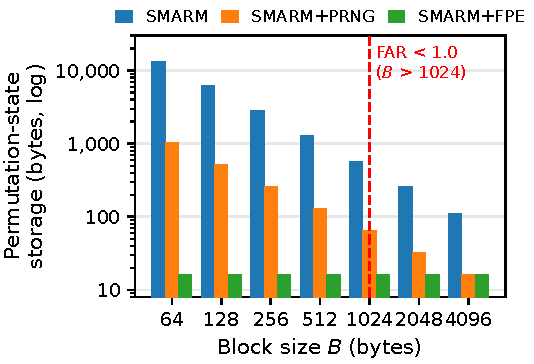
\includegraphics[width=0.85\linewidth]{fig_storage.pdf}
\caption{Secure storage requirement $|\sigma|$ for each scheme 
across block sizes $B$. The dashed red line marks 
$B = 1024$~bytes, beyond which baseline SMARM's FAR drops below 
$1.0$ (Chapter~\ref{ch:eval-smarm}). Both SMARM+ variants 
substantially reduce storage overhead relative to SMARM, with 
SMARM+FPE achieving a constant footprint 
independent of $B$.}
\label{fig:storage_tradeoff}
\end{figure}

Both SMARM+ variants substantially reduce secure-storage overhead 
relative to SMARM across all evaluated configurations. The 
magnitude of reduction varies across the two variants as $B$ 
changes:

For \textbf{SMARM+PRNG}, the storage benefit is 
greater when $n$ is large (equivalently, when $B$ is small). 
SMARM+PRNG achieves a $13\times$ reduction at 
$B = 64$ bytes ($13{,}312 \rightarrow 1{,}024$ bytes), while the 
reduction decreases to approximately $7\times$ at $B = 4096$ 
bytes ($112 \rightarrow 16$ bytes). This trend arises because 
both SMARM and SMARM+PRNG storage requirements 
scale with $n$, albeit with different asymptotic costs: 
$O(n \log n)$ vs $O(n)$.

For \textbf{SMARM+FPE}, the storage requirement 
is a fixed $16$ bytes for FFX key material, independent of $B$ 
or $n$. As a result, SMARM+FPE achieves 
increasingly larger reductions as $B$ decreases. At $B = 64$ 
bytes, SMARM+FPE provides an $832\times$ 
reduction compared to SMARM, far exceeding 
SMARM+PRNG. As $B$ increases, the relative 
benefit narrows, and both variants provide comparable storage 
savings at large block sizes such as $B = 4096$ bytes.

\textbf{Key observation at the real-time boundary.} At $B = 
1024$ bytes — the boundary block size for SMARM baseline 
real-time compatibility — SMARM+PRNG reduces 
storage from $576$ bytes to $64$ bytes ($9\times$ reduction), 
while SMARM+FPE further reduces it to $16$ 
bytes ($36\times$ reduction).

\subsubsection{Overall Attestation Runtime}
\label{sec:smarmplus-runtime-eval}

Table~\ref{tab:runtime_overhead} reports the absolute attestation 
runtime for all three schemes, and 
Figure~\ref{fig:runtime_overhead} presents the runtime overhead 
of the SMARM+ variants relative to SMARM.

% [TABLE 1 - ดึงจาก journal Table I]
\begin{table}[H]
\centering
\caption{Overall attestation runtime of SMARM baseline and the 
two SMARM+ variants across block sizes. The shaded row 
($B = 1024$ bytes) marks the largest block size for which SMARM 
baseline maintains FAR~$\approx 1.0$.}
\label{tab:runtime_overhead}
\begin{tabular}{rrrr}
\toprule
& \multicolumn{3}{c}{\textbf{Runtime (ms)}} \\
\cmidrule(lr){2-4}
\textbf{$B$ (bytes)} 
& \textbf{SMARM} 
& \textbf{SMARM+PRNG} 
& \textbf{SMARM+FPE} \\
\midrule
64    & 644 & 9{,}310 & 4{,}229 \\
128   & 562 & 2{,}730 & 2{,}325 \\
256   & 521 & 1{,}066 & 1{,}423 \\
512   & 500 &   630   &   945   \\
\rowcolor{gray!15}
1024  & 490 &   526   &   726   \\
2048  & 484 &   494   &   611   \\
4096  & 481 &   484   &   553   \\
\bottomrule
\end{tabular}
\end{table}

% [FIG 4 - ดึงจาก journal: fig_runtime_overhead.pdf ใช้ตรงๆได้เลย]
\begin{figure}[H]
\centering
\includegraphics[width=0.85\linewidth]{fig_runtime_overhead.pdf}
\caption{Overall runtime overhead of SMARM+PRNG 
and SMARM+FPE relative to the SMARM baseline 
across block sizes. The dashed red line marks $B = 1024$ bytes.}
\label{fig:runtime_overhead}
\end{figure}

The results reveal two distinct overhead patterns:

\textbf{SMARM+PRNG overhead grows steeply for 
small $B$.} The bitmap-based block selection requires scanning 
$O(n)$ entries per iteration. Since $n$ grows inversely with $B$, 
the cumulative scan cost across $n$ iterations is $O(n^2)$, 
becoming dominant at small block sizes. At $B = 64$ bytes, 
SMARM+PRNG incurs a $13.5\times$ runtime increase 
(9{,}310 ms vs 644 ms), making it impractical for configurations 
requiring very small block sizes.

\textbf{SMARM+FPE overhead is more moderate but 
non-zero.} The FFX operation has $O(1)$ runtime complexity, but 
each invocation requires multiple Speck rounds — more expensive 
than a single bitmap scan when $n$ is small. As a result, 
SMARM+FPE is faster than 
SMARM+PRNG at $B \leq 128$ bytes but slower at 
$B \geq 256$ bytes.

\textbf{At the real-time boundary ($B = 1024$ bytes).} 
SMARM+PRNG incurs only $7\%$ runtime overhead 
(526 ms vs 490 ms), while SMARM+FPE incurs 
$48\%$ overhead (726 ms vs 490 ms). At this block size, the 
overall runtime is dominated by HMAC-SHA256 computation over 
the memory blocks, so the additional per-iteration overhead of 
both variants contributes only a modest fraction of the total.


\subsubsection{Real-Time Availability Verification}
\label{sec:smarmplus-far-eval}

A key concern is whether the modified permutation representations 
in SMARM+ affect real-time behavior. Recall from 
Chapter~\ref{ch:eval-smarm} that FAR is governed primarily by 
$t_{\mathrm{disabled}}$ per block — the time interrupts remain 
disabled during a single block measurement.

Both SMARM+ variants preserve this $t_{\mathrm{disabled}}$ 
unchanged: the atomic measurement step (HMAC.Update under 
disabled interrupts) is identical across SMARM, 
SMARM+PRNG, and SMARM+FPE. The 
additional computations introduced by SMARM+ (bitmap scan, FFX 
encryption) execute \emph{outside} the atomic critical section, 
with interrupts enabled. We therefore expect FAR behavior of 
SMARM+ to closely follow the baseline established in 
Chapter~\ref{ch:eval-smarm}.

To verify this empirically, we measured FAR for both SMARM+ 
variants under low, medium, and high real-time workloads on both 
FreeRTOS and Zephyr, using the same protocol as 
Chapter~\ref{ch:eval-smarm}. Figure~\ref{fig:far_smarmplus} 
reports the results.

\begin{figure}[H]
    \centering
    \includegraphics[width=\linewidth]{far_smarmplus_combined.pdf}
    \caption{FAR of SMARM, SMARM+PRNG, and 
    SMARM+FPE across block sizes 
    $B \in \{64, \ldots, 4096\}$ bytes, under three real-time 
    workload classes (columns) on FreeRTOS (top row) and 
    Zephyr (bottom row). All three schemes preserve 
    FAR~$\approx 1.0$ for $B \leq 1024$ bytes across all 
    configurations. At $B \geq 2048$ bytes, the SMARM+ variants 
    follow the same degradation pattern as baseline SMARM, 
    confirming that the bitmap scan 
    (SMARM+PRNG) and FFX encryption 
    (SMARM+FPE) introduced outside the atomic 
    critical section do not alter the real-time interference 
    characteristics of the scheme.}
    \label{fig:far_smarmplus}
\end{figure}

The results confirm our analytical expectation. For 
$B \leq 1024$ bytes, all three schemes achieve FAR~$=1.0$ 
across all six configurations (3 workloads $\times$ 2 RTOSes). 
For $B \geq 2048$ bytes, all three schemes degrade together: 
the curves overlap closely, with SMARM+FPE 
sitting slightly above the baseline and SMARM+PRNG 
sitting almost on top of it. For example, at the high-frequency 
workload (1000~Hz) on FreeRTOS, the SMARM baseline drops to 
FAR~$\approx 0.54$ and $0.28$ at $B = 2048$ and $4096$ 
respectively; SMARM+PRNG drops to $0.54$ and 
$0.28$, while SMARM+FPE drops to $0.62$ and 
$0.33$. The same trend holds on Zephyr, where the baseline drops 
to $0.63$ and $0.32$ while SMARM+PRNG drops to 
$0.64$ and $0.32$, and SMARM+FPE drops to $0.67$ 
and $0.39$.

The slightly higher FAR observed for SMARM+FPE at 
large block sizes is consistent with its longer overall 
attestation runtime (Table~\ref{tab:runtime_overhead}): the 
additional FFX encryption performed outside the atomic critical 
section extends the interrupt-enabled windows between consecutive 
block measurements, giving the real-time task more opportunities 
to preempt the Wrapper Task. The effect is more visible at the 
low-frequency workload (10~Hz, $B=2048$), where SMARM+ variants 
register slightly lower FAR than the baseline — an artifact of 
the longer overall runtime spreading missed deadlines over more 
task periods rather than a deeper interruption issue.

These observations confirm that the FAR behavior of both SMARM+ 
variants is governed entirely by $t_{\mathrm{disabled}}$ per 
block — which remains unchanged from baseline SMARM — rather than 
by the additional computation introduced outside the atomic 
critical section. SMARM+ therefore preserves SMARM's real-time 
properties: it neither improves nor degrades them.

\subsection{Trade-off Analysis and Deployment Guidance}
\label{sec:smarmplus-deployment}

The results of Section~\ref{sec:smarmplus-eval} reveal that 
SMARM, SMARM+PRNG, and SMARM+FPE 
occupy distinct points on the storage-vs-runtime trade-off curve. 
No single scheme is universally best; the choice depends on the 
deployment scenario the designer is facing. In this section, we 
frame the choice as a sequence of practical questions that 
correspond to the use cases addressed by this thesis.

\subsubsection{Use-Case 1: Real-time deadlines are violated}

\textbf{Symptom.} The system runs SMARM at the block size 
demanded by its secure-storage budget, but real-time tasks 
miss their deadlines (FAR~$\ll 1.0$ at $B \geq 2048$ bytes).

\textbf{Cause.} The non-interruptibility period 
$t_{\mathrm{disabled}}$ exceeds the period of the time-sensitive 
task. As established in Chapter~\ref{ch:eval-smarm}, this occurs 
whenever the SHA-256 hash over a single block takes longer than 
one task period — i.e., for $B \geq 2048$ bytes at 110~MHz on 
our target platform.

\textbf{Recommendation.} Apply the \emph{atomic copy enhancement} 
(Chapter~\ref{ch:atomic-copy}). It reduces $t_{\mathrm{disabled}}$ 
by approximately $15$--$71\times$ by shifting the atomic 
operation from cryptographic hashing to memory copy, restoring 
FAR~$\approx 1.0$ at any block size up to 4096~bytes.

\textbf{Trade-off.} Negligible. The atomic copy enhancement adds 
no extra secure storage and only marginal additional computation 
(one memcpy per block before each HMAC update).

\subsubsection{Use-Case 2: Secure RAM cannot fit the permutation}

\textbf{Symptom.} The block size needed for real-time 
compatibility ($B \leq 1024$ bytes) produces a permutation 
$\sigma$ that exceeds the available Secure RAM, or competes with 
other security-critical services (e.g., confidential 
inference~\cite{islam2023confidential}, 
CFI~\cite{kawada2021tzmcfi}, key 
storage~\cite{silabs2020an1271}).

\textbf{Cause.} Baseline SMARM stores $\sigma$ explicitly, with 
$|\sigma| = n \cdot \lceil \log_2 n \rceil$ bits. At 
$B = 1024$ bytes this is 576~bytes; at $B = 64$ bytes it grows 
to approximately 13~KB.

\textbf{Recommendation.} Apply one of the two SMARM+ variants. 
The choice depends on how tight the Secure-RAM budget is, and 
how much additional attestation runtime is acceptable:

\begin{itemize}
    \item \textbf{SMARM+PRNG} reduces storage to 
    $O(n)$ bits via a bitmap. At $B = 1024$ bytes, this gives a 
    $9\times$ storage reduction (576~B $\rightarrow$ 64~B) at 
    only $7\%$ additional runtime. Recommended when 
    Secure~RAM is moderately constrained and runtime overhead 
    must be minimized.
    
    \item \textbf{SMARM+FPE} eliminates 
    permutation storage entirely ($O(1)$ bits, 16~bytes for 
    FFX key material). At $B = 1024$ bytes, this gives a 
    $36\times$ storage reduction at $48\%$ additional 
    runtime. Recommended when Secure~RAM is heavily contended 
    and attestation runtime is not on the critical path.
\end{itemize}

\textbf{Trade-off.} Reduced secure-storage footprint comes at 
the cost of additional per-block computation (bitmap scan or 
FFX encryption). Importantly, neither variant changes 
$t_{\mathrm{disabled}}$, so real-time behavior 
(Section~\ref{sec:smarmplus-far-eval}) is preserved.

\subsubsection{Use-Case 3: Neither real-time nor storage is constrained}

\textbf{Symptom.} The system has ample Secure~RAM dedicated to 
attestation, and the chosen block size already meets real-time 
requirements.

\textbf{Recommendation.} Baseline SMARM. It has the simplest 
design, the lowest runtime overhead, and incurs no per-block 
computation beyond hashing. The atomic copy enhancement and 
SMARM+ variants offer no benefit in this scenario.

\subsubsection{Summary of Recommendations}

Table~\ref{tab:deployment_scenarios} summarizes the use cases 
and recommended schemes.

\begin{table}[H]
\centering
\caption{Use-case-based selection guide for SMARM, SMARM+PRNG, 
and SMARM+FPE, and the atomic copy enhancement.}
\label{tab:deployment_scenarios}
\small
\begin{tabular}{p{4.0cm}p{3.6cm}p{6.0cm}}
\toprule
\textbf{Scenario you are facing} & \textbf{Recommended} 
& \textbf{Why} \\
\midrule
Real-time deadlines are missed at large block sizes 
& Atomic copy 
(Chapter~\ref{ch:atomic-copy}) 
& Reduces $t_{\mathrm{disabled}}$ by 15--71$\times$; FAR 
restored to $\approx 1.0$ at any block size. \\
\addlinespace
Secure RAM is moderately constrained 
& SMARM+PRNG 
& 9--13$\times$ storage reduction with only 7--26\% extra 
runtime at $B \geq 512$ bytes. \\
\addlinespace
Secure RAM is heavily contended (multi-service Secure world) 
& SMARM+FPE 
& Constant 16-byte footprint regardless of block size; 
36--832$\times$ storage reduction. \\
\addlinespace
No real-time or storage pressure 
& SMARM (baseline) 
& Simplest design, lowest runtime; no need for additional 
mechanisms. \\
\bottomrule
\end{tabular}
\end{table}


\subsection{Summary}
\label{sec:smarmplus-summary}

This chapter proposed SMARM+, a family of storage-efficient SMARM 
variants designed to address the secure-storage bottleneck 
identified in Chapter~\ref{ch:atomic-copy}. 
SMARM+PRNG replaces the explicit permutation 
array with an $n$-bit bitmap, reducing storage from 
$O(n \log n)$ to $O(n)$ bits, while 
SMARM+FPE eliminates permutation storage 
entirely via format-preserving encryption, requiring only 
$O(1)$ secure memory.

At the real-time boundary block size ($B = 1024$ bytes), 
SMARM+PRNG achieves a $9\times$ storage reduction 
with only $7\%$ runtime overhead, while 
SMARM+FPE achieves a $36\times$ reduction at 
$48\%$ additional runtime. Both variants preserve SMARM's 
security guarantees (S1)--(S3) and inherit the real-time 
behavior of the baseline.

SMARM+ addresses the secure-storage dimension of SMARM's 
deployability problem, which is orthogonal to the real-time 
dimension addressed by the atomic copy enhancement of 
Chapter~\ref{ch:atomic-copy}. Together, the two contributions 
cover the distinct deployment scenarios encountered on 
resource-constrained TrustZone-M devices, as discussed in the 
deployment guidance of Section~\ref{sec:smarmplus-deployment}.



\section{Conclusion}
\label{ch:conclusion}

This thesis investigated the coexistence of remote attestation and 
real-time availability on resource-constrained TrustZone-M devices. 
Starting from the observation that traditional remote attestation 
techniques require non-interruptible memory measurements that 
conflict with real-time workloads, we systematically examined how 
shuffled-measurement attestation — specifically SMARM — can be 
adapted, evaluated, and enhanced for practical deployment on 
RTOS-driven IoT platforms.

\subsection{Summary of Contributions}
\label{sec:contributions-summary}

This thesis makes four contributions, presented across 
Chapters~\ref{ch:methodology}--\ref{ch:smarmplus}:

\paragraph{Contribution 1: TrustZone-M-based SMARM realization 
(Chapter~\ref{ch:methodology}).}
We presented the first realization of SMARM on commodity ARM 
TrustZone-M hardware, replacing the formally verified seL4 
microkernel of the original HYDRA-based prototype. Our design 
decomposes SMARM into a Non-Secure Wrapper Task and a Secure 
Service connected via NSC entry points, preserving SMARM's 
original security guarantees (S1)--(S3) through hardware-enforced 
isolation rather than software-level verification. The prototype 
implementation supports both FreeRTOS and Zephyr on the 
STM32L552ZE platform with a Secure-world TCB of $33{,}968$ bytes.

\paragraph{Contribution 2: Systematic real-time evaluation 
(Chapter~\ref{ch:eval-smarm}).}
We conducted the first systematic evaluation of SMARM under 
real-time workloads and introduced the \emph{Frequency Accuracy 
Ratio} (FAR) as a quantitative metric for real-time compatibility. 
Our evaluation revealed a fundamental limitation: SMARM maintains 
FAR~$\approx 1.0$ only for block sizes $B \leq 1024$ bytes, while 
larger blocks degrade real-time availability significantly 
(FAR~$\approx 0.27$ at $B = 4096$ bytes under high-frequency 
workloads). FreeRTOS and Zephyr yield nearly identical results, 
confirming that the interference is governed by the block 
measurement itself rather than RTOS-specific scheduling behavior.

\paragraph{Contribution 3: Atomic copy enhancement 
(Chapter~\ref{ch:atomic-copy}).}
We proposed shifting the atomic operation from cryptographic 
hashing to memory copy, recognizing that what must be protected 
atomically is the \emph{capture} of the block, not its hashing. 
This enhancement reduces $t_{\mathrm{disabled}}$ by approximately 
$15$--$71\times$ across all evaluated block sizes and restores 
FAR to $\approx 1.0$ at every block size up to $4096$ bytes, 
effectively eliminating the real-time bottleneck of SMARM.

\paragraph{Contribution 4: SMARM+ for storage-efficient attestation 
(Chapter~\ref{ch:smarmplus}).}
We proposed two enhanced variants that address the orthogonal 
secure-storage limitation revealed by the atomic copy enhancement:

\begin{itemize}
    \item \textbf{SMARM+PRNG} reduces secure 
    storage from $O(n \log n)$ to $O(n)$ bits using a compact 
    bitmap and PRNG-based block selection. At the real-time 
    boundary block size ($B = 1024$ bytes), it achieves a 
    $9\times$ storage reduction at only $7\%$ additional runtime.
    
    \item \textbf{SMARM+FPE} eliminates 
    permutation storage entirely (to $O(1)$ bits) by deriving 
    the measurement order on-the-fly via format-preserving 
    encryption based on the FFX construction with the Speck 
    cipher. It achieves a $36\times$ storage reduction at 
    $B = 1024$ bytes, at the cost of $48\%$ additional runtime.
\end{itemize}

Both variants preserve the security guarantees (S1)--(S3) of 
SMARM and are orthogonal to the atomic copy enhancement.

\subsection{Deployment Guidance}
\label{sec:deployment-guidance}

A central question for practitioners is: \emph{given my hardware 
constraints and workload, which of the proposed mechanisms 
should I deploy?} Our evaluation suggests that the answer is 
best framed as a sequence of independent decisions, since the 
atomic copy enhancement and the SMARM+ variants address two 
distinct problems and need not be applied together.

\paragraph{Decision 1: Does the system have real-time tasks 
whose deadlines are missed under baseline SMARM?}
If yes, the atomic copy enhancement should be applied. It 
reduces $t_{\mathrm{disabled}}$ by approximately 
$15$--$71\times$ and restores FAR~$\approx 1.0$ at any block 
size, at negligible additional cost. If real-time tasks are 
already met (either because the system is not real-time, or 
because the chosen block size already satisfies real-time 
constraints), this enhancement is unnecessary.

\paragraph{Decision 2: Does the permutation array fit comfortably 
within the available Secure~RAM?}
If yes, baseline SMARM is the simplest and most 
runtime-efficient choice. If no — for example, when Secure RAM 
is shared with confidential 
inference~\cite{islam2023confidential}, control-flow integrity 
monitoring~\cite{kawada2021tzmcfi}, or secure key 
storage~\cite{silabs2020an1271} — one of the SMARM+ variants 
should be applied:

\begin{itemize}
    \item \textbf{SMARM+PRNG} is preferred when 
    Secure RAM is moderately constrained and attestation runtime 
    must be kept low. At $B \geq 512$~bytes, it achieves 
    $9$--$10\times$ storage reduction with only $7$--$26\%$ 
    runtime overhead.
    
    \item \textbf{SMARM+FPE} is preferred when 
    Secure RAM is heavily contended and attestation latency is 
    not the bottleneck. Its constant-size footprint enables 
    coexistence with other security-critical services regardless 
    of block size.
\end{itemize}

We emphasize that Decisions~1 and~2 are independent: a system 
might apply atomic copy alone (real-time-critical but 
storage-unconstrained), SMARM+ alone (storage-constrained but 
not real-time-critical), or neither (neither constrained). The 
question of how to combine these two mechanisms into a single 
unified scheme — and whether such combination yields additional 
benefit — is left as future work 
(Section~\ref{sec:future-work}).

\subsection{Limitations}
\label{sec:limitations}

Despite the contributions above, this thesis has several 
limitations worth noting.

\paragraph{Real-time evaluation is necessary but not sufficient.}
FAR captures the extent to which a real-time task maintains its 
intended execution frequency under attestation-induced 
interference. However, FAR~$\approx 1.0$ does not, on its own, 
guarantee full schedulability. Worst-case execution time (WCET) 
analysis, deadline miss rate, and response-time analysis under 
multi-task workloads are required to formally certify a system 
for hard real-time deployment. Such analysis is orthogonal to 
our study and was deliberately scoped out.

\paragraph{Single real-time task.}
Our evaluation considers a simplified scenario with a single 
real-time task $T_{RT}$ at varying frequencies. While this 
provides a clear conservative baseline — if coexistence fails 
here, it would also fail in more complex settings — real 
deployments typically involve multiple tasks with different 
priorities and deadlines. The scheduling interference patterns 
in such systems may differ from our single-task setup.
Furthermore, we do not analyze the cumulative RTOS time drift
that can arise from atomic Secure-world execution;
this orthogonal issue is characterized in
detail in~\cite{joianeto2026iccad}, and combining their
SysTick compensation mechanism with our SMARM enhancements
is a promising direction for future work.

\paragraph{FPE small-domain considerations.}
SMARM+FPE relies on the FFX construction, which 
is theoretically vulnerable to small-domain 
attacks~\cite{hoang2018curse} when an adversary can observe or 
query plaintext-ciphertext pairs. We argued in 
Chapter~\ref{ch:smarmplus} that the attack preconditions do not 
arise in our setting — the ciphertext outputs (block indices) 
remain confined to Secure RAM, and no oracle access is exposed 
to untrusted code. Nonetheless, hardening 
SMARM+FPE against side-channel leakage of 
internal indices remains an open consideration for 
deployments where such leakage cannot be precluded.

\paragraph{Single hardware platform.}
Our implementation and evaluation are conducted on a single 
TrustZone-M platform (STM32L552ZE Nucleo-144 with Cortex-M33 at 
110 MHz). The absolute timing results — both 
$t_{\mathrm{disabled}}$ values and attestation runtime — will 
vary across platforms with different memory bus speeds, CPU 
frequencies, and Secure-world TCB sizes. The relative 
relationships among the schemes (ratios, trends, trade-off 
boundaries) should generalize, but absolute performance 
predictions for other platforms require platform-specific 
measurement.

\paragraph{Threat model scope.}
Following SMARM's threat model, we consider software-level 
adversaries with full control over the Non-Secure world but 
treat hardware attacks, physical attacks, side-channel attacks, 
and denial-of-service attacks as out of scope. These attack 
classes may apply to TrustZone-M deployments in practice and 
warrant separate study in their own threat models.

\subsection{Future Work}
\label{sec:future-work}

Two directions naturally extend the work presented in this 
thesis.

\paragraph{Combining atomic copy with SMARM+ variants.}
The atomic copy enhancement (Chapter~\ref{ch:atomic-copy}) and 
the SMARM+ variants (Chapter~\ref{ch:smarmplus}) address 
orthogonal limitations of SMARM. In principle, they can be 
combined: replacing the atomic HMAC update of 
SMARM+PRNG or SMARM+FPE with 
the two-step \texttt{Memcpy} + interrupt-enabled hash pattern 
would yield a scheme that is simultaneously real-time-compatible 
across all block sizes and storage-efficient. We did not 
evaluate this combination in this thesis since each contribution 
already provides a complete solution for its respective use 
case (real-time violation, or secure-storage shortage). 
Implementing and evaluating the combined scheme — including 
verifying that real-time and storage benefits compose 
additively without interference — is an interesting direction 
for future work.

\paragraph{Schedulability analysis.}
As discussed in Chapter~\ref{ch:eval-smarm}, the Frequency 
Accuracy Ratio (FAR) used in our evaluation is a necessary 
condition for real-time compatibility but does not, on its own, 
guarantee that real-time tasks will consistently meet their 
deadlines. A complete schedulability analysis, including metrics 
such as deadline miss rate, response time, and worst-case 
execution time (WCET), is orthogonal to our current study and 
is left for future work.

\paragraph{Combining shuffled measurements with other interruptible
attestation techniques.} As reviewed in Chapter~\ref{ch:literature},
several alternative approaches relax the atomicity requirement of
traditional remote attestation through different design strategies.
Self-measurement techniques~\cite{erasmus, reconciling-ra, iterator}
allow the prover to initiate attestation independently of the verifier,
enabling measurements to be scheduled at times that minimize interference
with real-time tasks. Interrupt vector table attestation
schemes~\cite{isc-flat, asap, pistis} permit interrupts during attestation
by additionally measuring the IVT, based on the intuition that malicious
interrupt-driven behavior will be reflected in the attestation evidence.
Hardware-assisted memory monitoring approaches~\cite{lo-fat, litehax,
atrium, perfcounter-ra} use dedicated hardware support to reduce or
eliminate non-interruptible execution windows. These alternatives are
complementary to shuffled measurements; investigating how they can be
combined with SMARM+ to jointly improve security and real-time
compatibility is an interesting direction for future work.

\paragraph{Integrating SysTick drift compensation.}
As discussed in Section~\ref{sec:limitations}, atomic Secure-world
execution can cause cumulative time drift in the Non-Secure RTOS,
a problem studied by Joia Neto et al.~\cite{joianeto2026iccad}.
Their Secure-driven SysTick compensation mechanism corrects this
drift by updating the RTOS time-keeping structures from the Secure
World during atomic execution. Combining this mechanism with
SMARM+ would address both the per-block non-interruptibility
studied in this thesis and the cumulative drift that can arise
in long-running deployments, yielding a more comprehensive
solution for real-time systems.

\subsection{Closing Remarks}
\label{sec:closing-remarks}

This thesis has shown that traditional remote attestation and 
real-time availability, although difficult to combine in 
practice, are not inherently incompatible on commodity 
TrustZone-M platforms. The conflict arises from two specific 
design choices in existing schemes: requiring atomic execution 
of the entire block hashing, and storing the measurement 
permutation as an explicit array in Secure RAM.

By disabling interrupts only during the memory copy rather than 
the full hash computation, the non-interruptibility period can 
be reduced by more than an order of magnitude. Independently, 
by representing the permutation using a bitmap or deriving it 
on-the-fly via format-preserving encryption, the secure-storage 
requirement can be reduced from $O(n \log n)$ to $O(n)$ or 
$O(1)$ bits. Together, the two contributions cover the 
distinct deployment scenarios encountered on resource-constrained 
TrustZone-M devices: real-time workloads on the one hand, and 
multi-service Secure-world deployments competing for Secure RAM 
on the other.

We hope this work provides a practical basis for deploying 
shuffled remote attestation in real-time IoT systems and that 
the design choices presented here will be useful for future 
attestation schemes targeting similar platforms.




\bibliographystyle{IEEEtran}
\bibliography{citation}

\end{document}


